%\documentclass[twoside,openright,a4paper,11pt]{book}
%
%
\usepackage[utf8]{inputenc}
\usepackage[francais]{babel}
\usepackage[T1]{fontenc}

\addto\captionsfrench{\def\tablename{\textsc{Tableau}}}% pour avoir TABLEAU et pas TABLE dans les légendes des tableaux

%%%%%%% MISE EN PAGES %%%%%%
\usepackage{geometry}
\geometry{outer=2cm,inner=3cm,top=3cm}

\setcounter{tocdepth}{3}     % Dans la table des matieres
\setcounter{secnumdepth}{3}  % Avec un numero.
\usepackage{setspace}

\usepackage{fancyhdr}	% marge en haut et en bas
\pagestyle{fancy}

\fancyhead{}	% vide l'entête
\fancyfoot{} % vide le pied~de~page

\fancyhead[RO]{\leftmark}
\fancyhead[LE]{\rightmark}
\fancyfoot[C]{\thepage}	% numéro de page en bas au centre

\renewcommand{\headrulewidth}{0.4pt} % épaisseur du trait en haut
\renewcommand{\footrulewidth}{0.4pt} % épaisseur du trait en bas

\fancypagestyle{mypagestyle}{%
    \fancyhead{}	
    \fancyfoot{} 
    \fancyfoot[C]{\thepage}
    \renewcommand{\headrulewidth}{0.4pt} 
	\renewcommand{\footrulewidth}{0.4pt} 
}

\fancypagestyle{couvertureAbstract}{%
    \fancyhead{}	
    \fancyfoot{} 
    \fancyfoot[C]{}
	\renewcommand{\headrulewidth}{0pt} 
	\renewcommand{\footrulewidth}{0pt} 
}
%
\usepackage{layout}
\usepackage{tocbibind} % include tableofcontent in itself

%%%%%% PAGE DE GARDE %%%%%%

\geometry{outer=2cm,inner=3cm,top=3cm}
\usepackage[scaled]{helvet} % font used on cover (Helvetica)
\usepackage{eso-pic} % to set background picture
\usepackage{multicol} % for back cover (abstracts)
\usepackage{graphicx} % to include logos
\usepackage{tikz} % to compose background picture

% Colors (extracted from SPI's template)
\definecolor{boxcolor1}{rgb}{0.91373,0.92941,0.87451}
\definecolor{boxcolor2}{rgb}{0.94902,0.93333,0.91373}
\definecolor{boxcolor3}{rgb}{0.76078,0.87843,0.17647}
\definecolor{headercolor}{rgb}{0.94118,0.30980,0.17255}
\definecolor{namecolor}{rgb}{1.0,0.4,0.0}
\definecolor{titlecolor}{rgb}{0.19216,0.51765,0.60784}
% Also used: gray, teal (predefined by xcolor package, usually loaded by document class)

% Cover environment, to keep changes local
\newenvironment{cover}{%
  \fontfamily{phv}\selectfont % Select Helvetica font
  \pagestyle{empty} % No page number
}{
  \addtocounter{page}{-1}
  \cleardoublepage
}

% Macro for background common to front and back
\newcommand{\tikzBG}{%
  \path (0,0) rectangle (1,1);
  %TODO: You should adjust the bottom height of the following rectangle to fit your abstract's length
  \path [fill=boxcolor1] (.0571,.11) rectangle (.481,.963); 
  \path [fill=boxcolor2] (.4333,.697) rectangle (.9048,.7475);
  \path [fill=boxcolor2] (.4333,.7811) rectangle (.9048,.8316);
  \path [fill=boxcolor2] (.4333,.8687) rectangle (.9048,.9192);
  \path [fill=boxcolor3] (.0571,.7879) rectangle (.5762,.8316);
  \node[inner sep=0pt] at (0.2285,0.8788) [above left] {%
    
\includegraphics[height=.0707\paperheight,keepaspectratio]{./figures/logo/logo_unb.png}};
  \node[inner sep=0pt] at (0.6667,0.8788) [above right] {%
    
\includegraphics[height=.0808\paperheight,keepaspectratio]{./figures/logo/logo_ecn_color.png}};
  \node at (.0571,.8316) [above right,color=headercolor] {%
    \fontsize{29}{35}\selectfont\bfseries Th\`ese de Doctorat};
}

% Macro for repeated information (to avoid insconsistency)
%TODO: fill in with no formatting but desired case
\newcommand{\firstName}{Jean-Rémy}
\newcommand{\surname}{Gloaguen}
\newcommand{\thesisTitle}{Estimation du niveau sonore de sources d'intérêts au sein de mixtures sonores urbaines : application au trafic routier}

%%%%%%% SYMBOLES %%%%%
\usepackage{tipa}	% pour avoir l'accent concave
\usepackage{lmodern}	% pour les guillemets
\usepackage{gensymb}	% pour les degrés
\usepackage{enumitem}	% pour changer le symbole de l'item (\begin{itemize}[label=$\bullet$])

%%%%%%% EQUATION %%%%%%
\usepackage{amssymb}
\usepackage{amsmath}
\usepackage{fancybox}
\usepackage{xfrac}	% fraction de type "1/4"
\usepackage{cases}	% système équation
\usepackage[overload]{empheq}
\usepackage{bm}		% pour mettre en gras .
\usepackage{units} 	% x/y barre latérale pour les fractions
%
%%%%%%% FIGURE %%%%%%
\usepackage{subfigure}	% utiliser subfigure
\usepackage{float}	% utiliser H dans les figures
%
%%%%%% TABLEAUX %%%%%%
\usepackage{array,multirow,makecell}
%\addto\captionsfrench{\def\tablename{\textsc{Tableau}}}% pour avoir TABLEAU et pas TABLE dans les légendes des tableaux
\usepackage{colortbl} % pour avoir des lignes colorées dans les tableau
%\usepackage{slashbox} % pour les \backslashbox
%\usepackage{subcaption}
\usepackage{hhline}	% pour les lignes horizontales 
\usepackage{tabularx} % permet itemize dans les cellules
\usepackage{booktabs}
\usepackage{longtable}	% pour les tableaux longs

\newcolumntype{L}[1]{>{\raggedright\let\newline\\\arraybackslash\hspace{0pt}}m{#1}}
\newcolumntype{C}[1]{>{\centering\let\newline\\\arraybackslash\hspace{0pt}}m{#1}}
\newcolumntype{R}[1]{>{\raggedleft\let\newline\\\arraybackslash\hspace{0pt}}m{#1}}

%%%%% ALGORITHME %%%%%
\usepackage{algorithm}
\usepackage{algorithmic}

%%%%% BIBLIO %%%%%
\usepackage[fixlanguage]{babelbib}
\selectbiblanguage{french}
\usepackage{breakcites}	% pour couper les références en bout de ligne

%%%%% APPENDICES %%%%%%%
\usepackage[toc,page]{appendix}

%%%%%%%%%%%%%%%%%%%%%
\usepackage{url}	% gérer les adresses www.
\linespread{1.2}	% interligne

\cleardoublepage
%
%\begin{document}

\chapter{Connaitre l'environnement sonore urbain : de la prédiction à la mesure}
\thispagestyle{empty}

\section{Pourquoi s'intéresser aux environnements sonores urbains ?}

Au sein de l'Union Européenne, 70 $\%$ de la population, soit quasiment 340 millions d'habitants, vivent dans des zones urbaines \cite{europ-commission_data_2017}. 486 villes concentrent, chacune, plus de 100 000 habitants. En France, selon l'INSEE, c'est même plus de 84 $\%$ de la population qui vivent dans une zone urbaine, soit plus de 55 millions d'habitants. Cette concentration soulève de grandes questions autour de l'organisation de l'espace urbain afin d'offrir une qualité de vie acceptable aux citadins. En effet, avec de telles densités (environ 3000 habitants/km$^2$ et jusqu'à plus de 21 000  habitants/km$^2$ pour la ville de Paris, la plus dense de l'UE), plusieurs formes de pollutions viennent dégrader l'environnement urbain. Des sources de désagrément perçues par le citadin, le bruit est le phénomène qui provoque le plus de gène après la pollution de l'air. Ce bruit est le fruit des activités humaines, provenant essentiellement du transport qu'il soit routier, ferroviaire ou aérien \cite{zannin_characterization_2013}.\\

Selon un rapport de l'Organisation Mondiale de la Santé (OMS) \cite{who_burden_2017}, en Europe, près de 200 millions de personnes sont exposées quotidiennement à des niveaux sonores supérieurs à 55 dB($A$), soit 40$\%$ de la population. Près de 20 $\%$ atteignent même plus de 65 dB($A$) en journée et plus de 30 $\%$ sont touchées par un niveau sonore excédant 55 dB($A$) la nuit. En France, selon un rapport de l'ADEME \cite{europeens2016analyse}, ce sont 52 millions de personnes qui se disent affectées par le bruit et principalement le bruit issu du trafic routier. Plus de 7 millions d'individus y sont alors exposés à des niveaux supérieurs à 65 dB($A$) au quotidien et à plus de 55 dB($A$) la nuit.
Cette exposition quotidienne, à de tels niveaux, n'est pas sans conséquence pour l'Homme. L'impact sur l'organisme humain à l'exposition du bruit est observé et étudié depuis de nombreuses années \cite{ising1980health}. Parmi les effets possibles, les plus courants sont des troubles du sommeil \cite{pirrera2010nocturnal}, de la vigilance et de la concentration, l'augmentation du stress, de la pression artérielle et du rythme cardiaque \cite{babisch2008road, babisch2005traffic}. Selon le rapport de l'OMS, ce sont près de 8 millions de personnes en Europe qui sont affectées par des troubles du sommeil mais aussi 900 000 touchées par de l'hypertension. On estime aussi que 43 000 hospitalisations sont imputables au bruit dues à des pertes de vigilance et de concentration et jusqu'à 10 000 cas de morts prématurées par an. Cet impact sur la santé a alors un coût financier pour la société : en France, ce coût est estimé à plus de 11,5 milliard d'euros par an dont une grande partie (89 $\%$) est imputable au bruit du trafic routier \cite{europeens2016analyse}. 

De plus, si le bruit en ville impacte la vie des citadins, celui-ci se fait également ressentir auprès de la faune sauvage \cite{dutilleux_anthropogenic_2012, francis2009noise} leur causant également du stress ou en compliquant la communication et la reproduction entre les individus.\\

Le bruit, et une trop grande exposition à celui-ci, a donc un impact négatif sur les individus et sur leur environnement. C'est donc un enjeu de société dont les français ont conscience \cite{JNA2016etude}. 
Il est donc nécessaire et utile de s'intéresser aux environnements sonores urbains (ESU) afin de mieux estimer les sources sonores présentes, leur niveaux sonores et leur répartition.
%  Étant la source sonore la plus présente et la plus gênante, de nombreuses études prises se sont focalisées sur le bruit de trafic.

De nombreux modèles numériques existent afin de pouvoir prédire les niveaux sonores émis par du trafic routier \cite{quartieri2009review}, ferroviaire \cite{van2000railway} et aérien \cite{zaporozhets1998aircraft}.
À partir de ces modèles, est instaurée en 2002, la directive européenne 2002/49/EC dont le but est de mieux connaitre la répartition du bruit émanant de ces principales sources de bruit en ville ainsi que des Installations Classées pour la Protection de l'Environnement (ICPE) dans les agglomérations de plus de 100 000 habitants. Cette directive prévoit : 

\begin{itemize}
	\item d'évaluer l'exposition au bruit des populations basée sur des méthodes communes aux pays européens,
	\item d'informer les populations sur leur niveau sonore d'exposition et sur les effets du bruit sur la santé,
	\item de connaitre et de délimiter les zones bruyantes et les zones calmes.\\
\end{itemize}

Cette directive permet notamment la production de cartes de bruits stratégiques qui permettent de cibler les endroits où les niveaux sonores sont élevés afin de réaliser des aménagements qui permettront de les réduire (construction d'un mur anti-bruit, réduction de la vitesse, mise en place d'un revêtement sol particulier \dots).


\section{Réaliser des cartes du bruit en ville}
Mises à jours tous les 5 ans, les cartes de bruit résument, pour chaque source de bruit, les niveaux sonores globaux moyens pondérés $A$ sur 24h ($L_{DEN}$ pour \textit{Day-Evening-Night}) et durant la nuit ($L_N$) : 

\begin{equation}
L_{DEN} = 10\times\log \left(\frac{1}{24} \left(12\times10^{\frac{L_D}{10}}+4\times10^{\frac{L_E+5}{10}}+8\times10^{\frac{L_N+10}{10}} \right)\right)
\end{equation} 

avec $L_D$, $L_E$ et $L_N$, les niveaux sonores moyens à long terme pondéré A pour les périodes respectives 6h-18h, 18h-22h, 22h-6h (pouvant être changer suivant le rythme de vie du pays), 

\begin{subequations}
\begin{align}
L_D &= 10\times\log\left(\frac{1}{T} \sum_{t = 1}^{T}10^{\frac{L_{D_t}}{10}}\right),\\
L_E &= 10\times\log\left(\frac{1}{T} \sum_{t = 1}^{T}10^{\frac{L_{E_t}}{10}}\right),\\
L_N &= 10\times\log\left(\frac{1}{T} \sum_{t = 1}^{T}10^{\frac{L_{N_t}}{10}}\right).
\end{align}
\end{subequations}

Les niveaux $L_E$ et $L_N$ sont majorés respectivement de 5 dB($A$) et de 10 dB($A$) afin de pénaliser les plages horaires où la gêne occasionnée par le trafic est plus importante. La Figure \ref{fig:carto_nantes} résume, par exemple, le $L_{DEN}$ et le $L_N$ pour le bruit du trafic routier dans un quartier de la ville de Nantes.

\begin{figure}[t]
\centering
\subfigure[\label{fig:lden}]{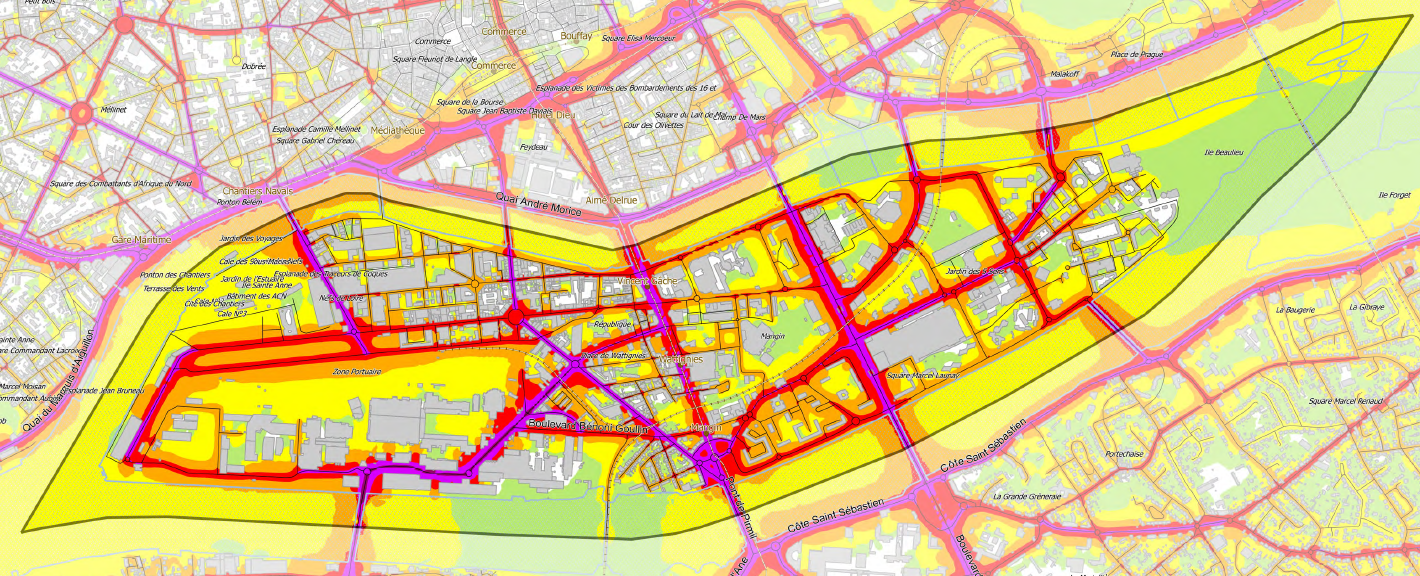
\includegraphics[width=0.85\linewidth]{./figures/cartographie/Lden_ile_Nantes.PNG}}
\subfigure[\label{fig:ln}]{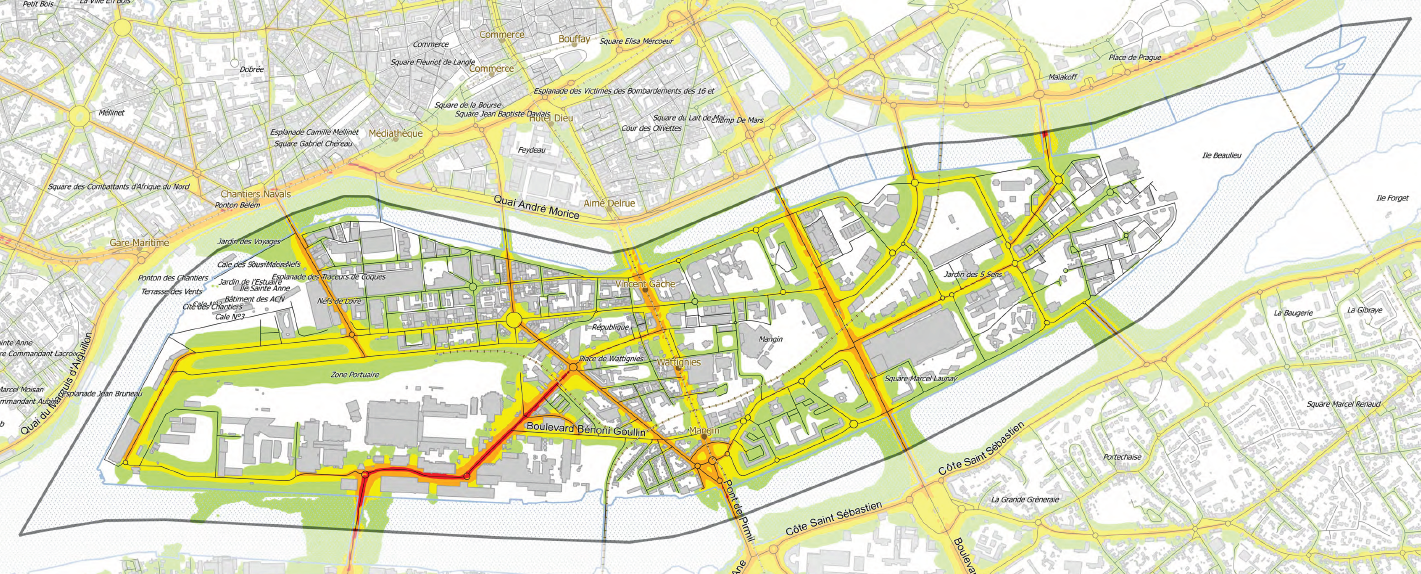
\includegraphics [width=0.7\linewidth]{./figures/cartographie/Ln_ile_Nantes.PNG}}
\caption{$L_{DEN}$ \subref{fig:lden} et $L_N$ \subref{fig:ln} de l'île de Nantes pour le trafic routier \cite{nantes_carte}.}
\label{fig:carto_nantes}
\end{figure}

Ces cartes sont issues de calculs numériques qui nécessitent de définir, comme données d'entrée, les caractéristiques des sources sonores et de l'environnement.  Dans le cas du trafic routier, cela revient à déterminer : 

\begin{itemize}
\item les vitesses moyennes des véhicules sur les portions de routes principales, 
\item les débits de véhicules (nombre de véhicules par tranche horaire \textit{Day, Evening, Night}), 
\item la composition du trafic (nombre de véhicules légers et de poids lourds).\\
\end{itemize}

Les lois d'émissions des sources sonores sont alors calculées. À partir de la topographie de la ville (architecture, revêtement du sol) et en obtenant les conditions météorologiques moyennes (température, vent), il devient possible de calculer, avec l'aide de modèles numériques de propagation acoustique, les niveaux sonores dans la ville produits par ces sources sonores. Plusieurs modèles existent comme le modèle NMPB-routes-2008 \cite{setra_prevision_2009-1, setra_prevision_2009-2},  CNOSSOS-EU \cite{CNOSSOS}, RSL-90\dots{} La génération des cartes peut être réalisée par des logiciels du commerce (comme Mithra, CadnaA ou Immi) qui font le choix d'utiliser un modèle de propagation parmi ceux existant. Actuellement, la méthode CNOSSOS-EU est l'approche la plus couramment utilisée à l'échelle de l'UE. Afin de déterminer, le nombre de citadins touchés par de forts niveaux sonores, les logiciels accompagnés d'un Système d'Information Géographique (SIG) sont ceux qui offrent le plus de possibilités. Un SIG est un outil informatique conçu pour stocker, analyser et manipuler plusieurs type de données spatiales et géographiques comme l'architecture des villes ou le nombre d'habitants présents. Leur utilisation permette de connaitre plus facilement le nombre de citadins exposés à des niveaux sonores \cite{murphy2011scenario}. Par exemple, le logiciel OrbisGIS\footnote{\url{http://orbisgis.org/}}, destiné à représenter de données spatiales, permet la réalisation de cartes de bruit à l'aide de l'ajout d'un plugin, \textit{NoiseModelling}, développé par \cite{fortin}. Un résumé des étapes est présenté en Figure \ref{fig:cartographie}.\\

\begin{figure}[t]
\centering
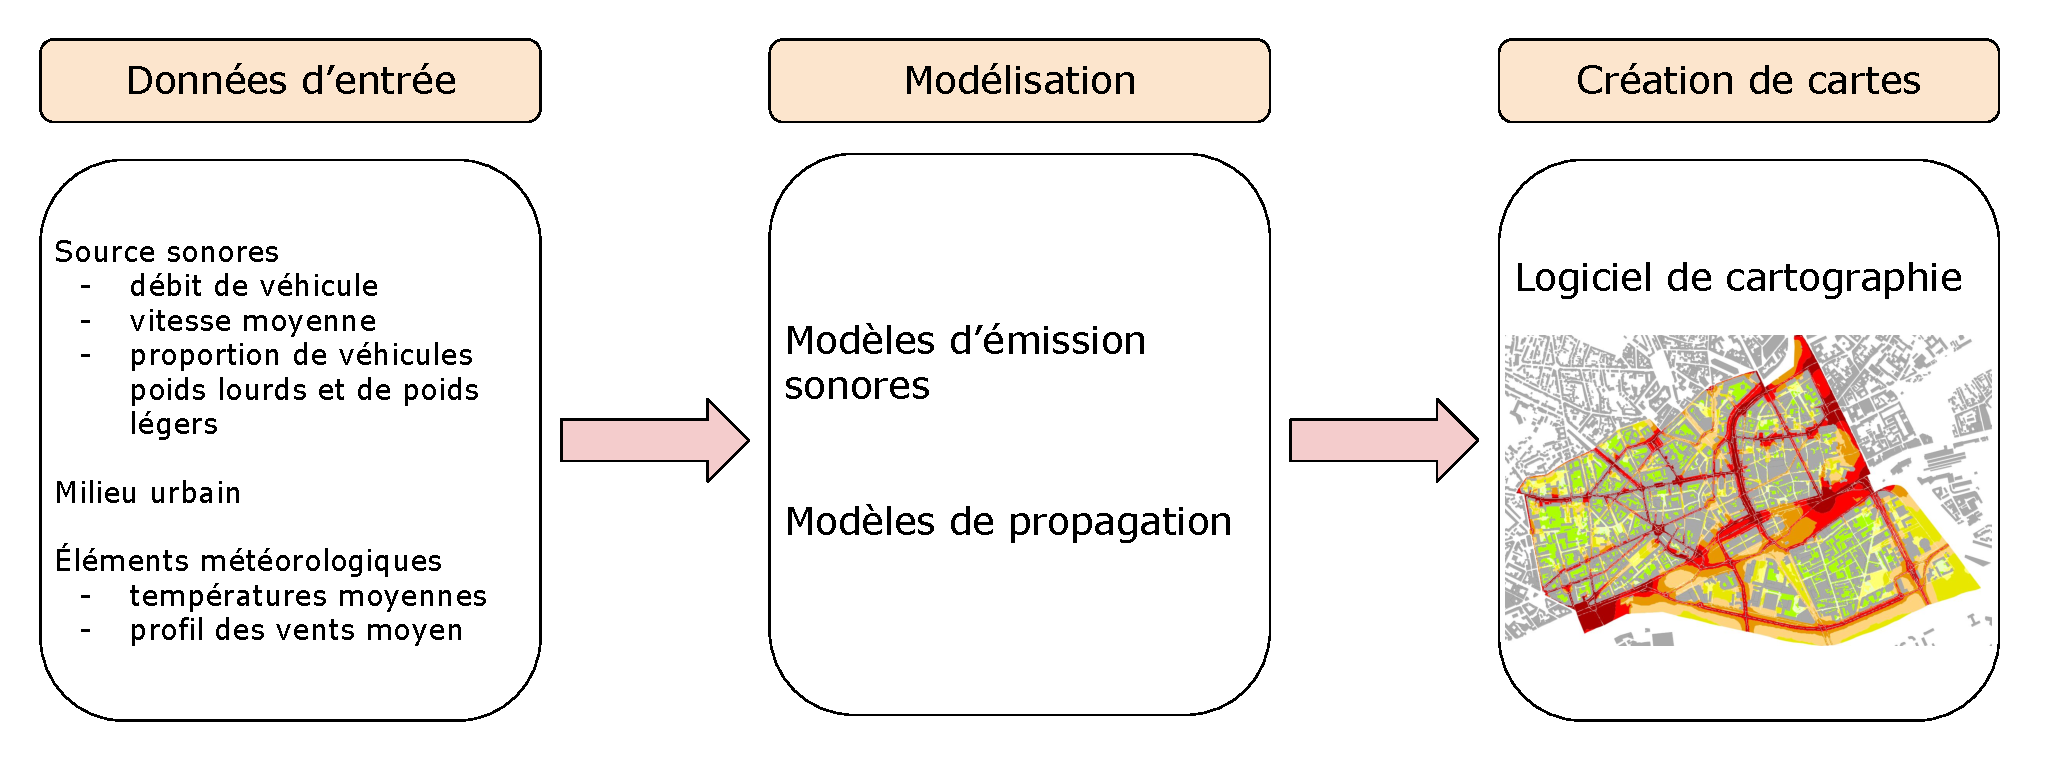
\includegraphics[width=.85\linewidth]{./figures/cartographie/cartographie.pdf}
\caption{Résumé des étapes menant aux cartes de bruit de trafic.}
\label{fig:cartographie}
\end{figure}


De nombreuses études basées sur l'étude du bruit en ville ou sur la réalisation de cartes de bruit dans des quartiers utilisent comme référence la directive européenne \cite{murphy_environmental_2006, murphy_estimating_2009, Eriksson_residential_2013}. Ces outils sont également utiles afin de tester différents scénarios d'aménagement (réduction de vitesse, changement de revêtements par exemple, construction d'immeuble \dots) \cite{murphy2011scenario,guedes2011influence}. Cependant, si l'utilité de ces cartes n'est pas remise en cause, chaque étape de la conception de ces cartes induit des incertitudes qui peuvent nuire à leur interprétation. 

\section{Limitations des modèles prédictifs de bruit de trafic}

\subsection{Incertitudes sur les données d'entrée}

La première source d'erreur est issue de l'estimation des données d'entrée à travers des valeurs moyennes qui induisent forcément des écarts types qui se propage par la suite aux étapes suivantes. 
Ensuite, le milieu urbain est évidemment simplifié pour éviter de complexifier et diminuer le temps de calcul. L'influence des plus petits mobiliers urbains est également mise de coté.
 

\subsection{Incertitudes des modèles physiques}

Ce type d'erreur est liée au choix de la méthode de calcul employée. Avant même la mise en place de la directive, Steele, dans \cite{steele_critical_2001}, avait comparé les méthodes de calculs (données d'entrée, type de cartographie, méthode de propagation des différents logiciels). Parmi cette diversité d'outils, l'auteur met en avant le problème, soulevé également par \cite{king_implementation_2011}, de la diversité des outils et des méthodes de calculs qui peuvent être employées. Plus récemment, Garg et Maji \cite{garg_critical_2014} réalisent une comparaison entre 8 méthodes de calcul (FHWA, CoRTN, RLS-90, ASJ RTN, Harmonoise, Son Road, Nord 2000n NMPB-Routes-2008) selon de nombreux points techniques : 

\begin{itemize}
\item modélisation des sources sonores (trafic, ferroviaire), 
\item condition de trafic (constantes, accélération/décélération, intersection\dots), 
\item modèle de propagation, 
\item prise en compte de la divergence géométrique, 
\item données d'entrées prise en compte, 
\item modélisation des effets de sol,
\item effets météorologiques,
\item effets de diffraction,
\item \dots  \\
\end{itemize}

Par exemple, la méthode RLS-90 est la seule à prédire la densité de trafic sur les axes routiers. La catégorisation des véhicules varie également entre les méthodes : dans la méthode Nord-2000, les véhicules sont divisés en 3 catégories selon leur poids alors que dans Son Road, il n'y en a que 2. Dans le cas du modèle de propagation, Harmonoise propose 3 méthodes (équation parabolique, tir de rayons et éléments de frontières) afin de s'adapter à différentes configurations là où, dans FHWA, c'est l'équation de propagation qui est résolue en prenant en compte les phénomènes comme l'absorption atmosphérique, les impédances des différentes surfaces rencontrées\dots{} Enfin les effets météorologiques sont pris différemment en compte selon les méthodes. La méthode NMPB suppose des conditions homogènes et favorables à la propagation. Dans Nord 2000, les gradients de température et de vent sont inclus alors que, dans les modèles Son Road et CoRTN, ces phénomènes ne sont pas pris en compte. L'ensemble des ces points amènent donc à des résultats divergeant entre les méthodes. 
Les auteurs concluent qu'il est toutefois difficile de déterminer un \og meilleur \fg{} modèle par rapport aux autres chacun ayant une approche différente. La validation de ces modèles par la mesure \textit{in situ} est complexe puisque de nombreuses sources sonores qui ne sont pas modélisées sont présentes en villes. 

Les premières cartes de bruits ont donc été établies sur des modèles différents. 
Afin de résoudre ces problèmes, la méthode CNOSSOS-EU \cite{CNOSSOS,kephalopoulos} a été développée. Même si elle présente certains défauts intrinsèques aux modèles prédictifs de bruit de trafic, elle permet d'harmoniser la construction des cartes de bruit des villes à l'échelle européenne permettant plus facilement leur comparaison. Dans le cas du trafic routier, la source sonore est décomposée selon 5 catégories de véhicule : légère, moyenne et lourde motorisation, 2 roues et autre. Cette dernière classe permet d'inclure, par exemple, les véhicules électriques. Les sources sonores sont décrites en prenant également en compte le bruit de roulement, de propulsion et les effets de l'accélération ou de décélération. 
La méthode de propagation choisie est celle des tirs de rayons. Entre la source et le récepteur, les chemins directs, réfléchis et diffractés sont considérés. En fonction des conditions atmosphériques relevées (température, vent), les atténuations dans les conditions favorables (à la propagation) et homogènes sont considérées. Les effets de sol (divisé en 8 catégories, du plus absorbant au plus réfléchissant), la divergence géométrique et l'absorption atmosphérique sont ensuite pris en compte. 

\subsection{Incertitudes liées à la modélisation numérique}

Les cartes de bruits étant simulées numériquement, des incertitudes apparaissent également liées à la modélisation et à la discrétisation du milieu urbain. Afin de limiter la durée des calculs, des techniques d'optimisation sont utilisées comme la discrétisation du milieu ou des sources de bruits. Par exemple, dans la méthode CNOSSOS, l'ensemble de l'émission sonore émise par une voiture est résumé en une source ponctuelle équivalente placé à 0,5 m du sol. Pour une route, considéré comme une source linéique de bruit, celle est discrétisée en un ensemble de sources ponctuelles alignées. Le choix de la distance entre ces points est alors un compromis à faire entre temps de calcul et la précision souhaitée. Toutefois la position de ces sources influe ensuite sur les phénomènes de réflexion et de diffraction et donc au résultat final. Enfin, entre ces sources ponctuelles, les niveaux sonores sont déterminés au moyen d'un calcul d'interpolation (linéaire, Kriging) qui viennent ajouter en plus des incertitudes \cite{van_leeuwen_noise_2015}. 
Également, toujours en vue de limiter la complexité des calculs, certains paramètres sont aussi ajustables comme le nombre de réflexion que subit un tir de rayon, ce qui a une influence directe sur l'établissement du champs diffus. 

\subsection{Incertitudes liées à la restriction d'informations}

Une des principales limites des modèles de bruits en ville est la restriction d'informations qu'elles proposent : 2 niveaux sonores, $L_{DEN}$ et $L_N$, par source de trafic, sont estimés et mis à jours seulement tous les 5 ans. Cependant, le trafic routier, ferroviaire et aérien varient aussi bien à l'échelle de l'année, d'une journée ou même d'une heure \cite{lv2015traffic}. 
L'utilisation de modèles dynamiques de trafic, couplé aux modèles d'émissions sonore  \cite{can2010traffic}, n'est actuellement pas destiné à la cartographie des ESU mais à l'étude des interactions entre les véhicules et à leur cinématique. 
Enfin, les modèles prédictifs de bruit ne sont actuellement pas validés \textit{in situ}. En effet, ces modèles de bruits actuel ne permettent d'estimer que les niveaux sonores des sources relatifs au trafic alors que le milieu urbain est composé d'une multitude de sources sonores qui ont une influence sur l'Environnement Sonore Urbain (abrégé ESU dans la suite du document) perçu par le citadin. De précédentes études \cite{Mioduszewski, zannin_characterization_2013} ont observé des différences significatives entre les niveaux sonores mesurés et calculés. Si ces différences peuvent provenir des inexactitudes générées par la simulation, une part de ces écarts proviennent de la présence d'autres sources sonores qui sont prises en comptes dans les mesures mais qui ne sont pas modélisées.\\ 

\section{Vers la modélisation d'autres sources sonores ?}

De nombreuse études se sont intéressées à l'étude des ESU à travers la perception qu'en ont les citadins (\cite{brocolini_measurements_2013},  \cite{hong2013designing}). La plupart de ces études définissent des grandeurs acoustiques (\textit{activité}, la \textit{clarté, l'évolution temporel, l'occupation spatiale}\dots) qui sont évalué sur des échelles de taille variables limités par des qualificatifs (respectivement \og monotone/varié \fg{}, \og brouhaha/distinct \fg{}, \og figée/évolutive \fg{}, \og peu présente/très présent \fg{} \dots) \cite{raimbault2003ambient}.
Une des difficultés est alors de lier les évaluations de ces grandeurs, lié au ressenti des gens, à des indicateurs physiques mesurables avec des instruments de mesures. 
Pour cela, certaines études se sont intéressées à corréler ces évaluations à des indicateurs physiques.
Dans \cite{torija2013application}, le paysage sonore est décrit, à partir d'écoutes réalisées en laboratoire, par 14 indicateurs physiques dont le facteur crête (rapport du niveau sonore maximum sur le niveau sonore équivalent à 15 minutes), le niveau sonore pondéré $A$ des signaux contenant une réponse impulsionnelle ou les niveaux sonores des bandes de tiers d'octave de 125 Hz et 16 kHz. 
Dans \cite{hong2014soundscape}, des cartes du paysage sonore urbain sont réalisées, à l'aide d'un logiciel SIG, à partir de l'évaluation perceptive de la présence du trafic, des sons technologiques, des sons humains et des sons naturels ainsi que de l'évaluation du paysage sonore et de l'environnement urbain. Ces évaluations sont complétées par un seul indicateur physique, le niveau sonore équivalent pondéré $A$, $L_{A,eq}$. Cette étude révèle que le bruit de trafic perçu est corrélé au $L_{A,eq}$ alors que les sons naturels (sifflement d'oiseaux, bruit de fontaine) ne le sont pas (corrélation négative). Dans \cite{aumond2017modeling}, c'est la notion d'agrément sonore qui est défini (ESU plaisant ou déplaisant) à partir de deux modèles : l'un physique et l'autre perceptif. Le modèle physique est basé sur des indicateurs physiques tels que le niveau sonore fractile $L_{50}$ dans la bande de tiers d'octave de 1 kHz ainsi que la variation normalisée en temps et en fréquence des bandes de 500 Hz et de 4 kHz. Le modèle perceptif est, quant à lui, établit à partir du niveau sonores globale et du temps de présence de plusieurs source sonore spécifiques : trafic, voix, et oiseaux. 
Ce modèle perceptif est intéressant car il ne lie pas la perception du citadins qu'à des indicateurs acoustiques mais avec, également, les temps de présence du trafic, des oiseaux et de la voix. Pour les estimer, l'utilisation des modèles prédictifs de bruit de trafic se révèlent donc insuffisants pour pouvoir compléter ce modèle perceptif en cela que la présence des oiseaux et de la foule sont inconnues. Or, leur modélisation \cite{hayne2011prediction} \cite{} ou celle d'autres sources, comme les fontaines \cite{watts2009measurement}, n'est, pour l'instant, que très peu étudiée.
De plus, la localisation de certaines de ces sources dans l'espace urbain reste difficile. En effet, les éléments trafic se concentrent sur des axes qui leur sont dédiés, l'estimation de leur débit est alors réalisable. Certaines sources sonores, comme les fontaines ou les cloches d'une église, étant fixes, sont aussi faciles à localiser. Mais les sources sonores, comme la foule et les oiseaux, sont plus difficiles à déterminer car plus mobiles et parcimonieuses. C'est donc plus par une approche statistique qu'on détermine les positions où ces sources sont le plus susceptibles de se trouver (sur des places ou sur les trottoirs pour les piétons, dans les parcs pour les oiseaux).\\

En conclusion, l'utilisation de modèles prédictifs existants ne permettent pas définir correctement les ESU et leur perception dans son ensemble. Ces modèles sont dédiés à un ensemble trop restrictif de sources sonores et présentent de nombreuses incertitudes. Afin de considérer l'ensemble des sources et des évènements sonores présents en ville et de compléter l'apport des modèles prédictifs, une autre approche est envisagée, basée sur la réalisation de mesures et d'enregistrements sonores. 

\section{Utilisation de mesures acoustiques}

À l'heure de l'émergence de l'\textit{Internet des choses} (ou \textit{Internet of Things} en anglais) \cite{zanella2014internet} et de la \textit{Smart City} \cite{chourabi2012understanding}, de nombreuses villes s'équipent actuellement en réseaux de différents types de capteurs disséminés dans le milieu urbain afin de mieux contrôler, en temps réel, de nombreux aspects de la ville : distribution d'énergie, gestion des transports, de l’eau ou des déchets. L'objectif étant alors d'optimiser le fonctionnement de la ville afin d'améliorer la qualité de vie des citadins.
L'intégration de capteurs acoustiques dans ces réseaux est alors une voie pour étudier les ESU dans leur globalité. Plusieurs approches ont été étudiées pour réaliser ces mesures à l'aide d'un ou de multiples capteurs, à partir de mesures fixes ou mobiles.

\subsection{Déploiement de réseaux de capteurs fixes}

Un des premier déploiement de capteurs consiste à installer à des positions définies des microphones professionnels pour une durée finie. Cette approche permet ainsi d'avoir accès aux variations à long terme des niveaux sonores à l'emplacement des microphones dont la position est connue et choisie spécifiquement. Un réseau de capteurs développé depuis plusieurs année est celui de la ville de Paris, géré par BruitParif, à travers le projet RUMEUR \cite{mietlicki2012innovative}, en région parisienne, qui existe déjà depuis plusieurs années où des réseaux de microphones sont déployés afin d'évaluer l'ESU en région parisienne. Un site internet\footnote{\url{http://rumeur.bruitparif.fr/}} est mis à disposition pour avoir un aperçu complet des mesures réalisées sur les nombreux sites. 
À une moindre échelle, plusieurs études se sont également intéressées à la réalisation de mesures de longue durée au sein de la ville. 
Dans \cite{Mioduszewski}, 40 microphones sont placés isolément à travers la ville de Gdansk en Pologne pour une durée d'un an afin de valider la cartographie de bruit. Dans \cite{zannin_characterization_2013}, 58 points de mesures qui sont déployés dans un campus universitaire de la ville de Curitiba au Brésil afin d'étudier son environnement sonore. Mais le coût de ces capteurs et leur maintenance restent élevés et leur déploiement dans un réseau dense à l'échelle d'une ville ou d'un quartier devient alors prohibitif. Grâce au développement de capteurs acoustiques à bas coûts \cite{van2010use}, il devient, aujourd'hui, envisageable de déployer un plus grand nombre de microphones à travers les villes pour des durées de mesures plus longues au détriment, certes, des performance individuelle de chaque capteur \cite{aumond2017study}. 

\begin{figure}[t]
\centering
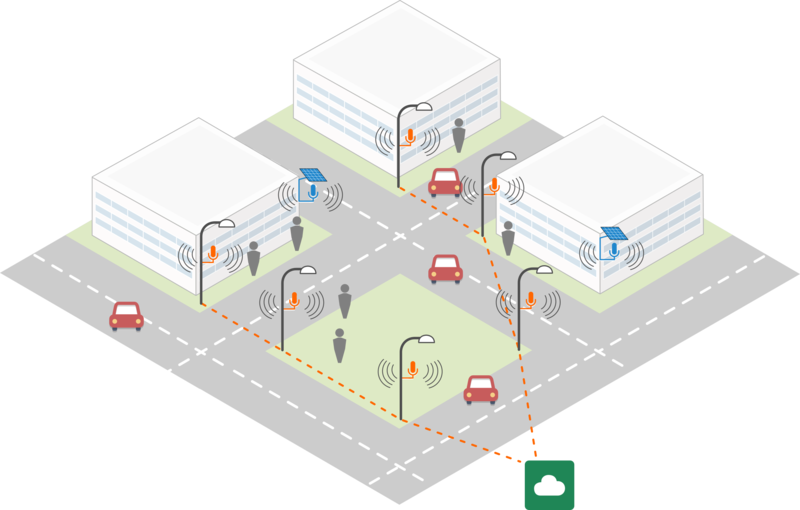
\includegraphics[width=0.8\linewidth]{./figures/cartographie/reseau_mesure.png}
\caption{Schéma d'un réseau de capteurs fixes}
\label{fig:reseau_capteur}
\end{figure}

\`A l'heure actuelle, plusieurs projets étudient la mise en place et la faisabilité de telle installation comme le projet européen DYNAMAP \footnote{\url{http://www.life-dynamap.eu/}} \cite{dynamap_2016}. Ce projet a pour objectif de développer un système de cartographie de bruit dynamique basé sur des réseaux de capteurs à bas coûts installés en ville. Une application de ce projet a déjà été réalisée dans deux villes tests, Milan et Rome \cite{bellucci_life_2017}. 

Le principe de leur approche est d'ajuster les cartes de bruits simulées à partir des différences obtenues entre les niveaux sonores mesurés aux stations et les niveaux sonores calculés à ce même point par les modèles prédictifs. Pour limiter le coût d'un tel déploiement, le nombre de microphones est réduit en les installant à des emplacements spécifiques représentatifs des différents scénarios possibles de trafic routier (homogénéité du trafic, type de revêtement, type de trafic\dots) \cite{zambon2017life}.
Le projet SONYC \footnote{\url{https://wp.nyu.edu/sonyc/}} à New-York dédie son réseau de capteurs à la surveillance de la pollution sonore et au développement d'outils de traitement du signal afin de décrire l'ESU par l'étude des sources présentes \cite{mydlarz2017noise}. Dans \cite{salamon2015unsupervised}, les auteurs classifient les évènements sonores à partir de leur base de données de sons, UrbanSound8k \cite{salamon_dataset_nodate}, avec, en tant que classifieur, un algorithme de k-moyenne sphérique.
Enfin, le projet CENSE\footnote{\url{http://cense.ifsttar.fr/}} vise à développer un réseau de capteurs dans la ville test de Lorient afin d'agréger les données simulées du niveaux sonores du trafic avec des mesures réalisées en ville par ce réseau en vue, là encore d'améliorer la cartographie du bruit de trafic. L'approche est différente de DYNAMAP, puisqu'ici l'étude se restreint à l'échelle de plusieurs quartiers de la ville afin d'avoir un réseau de capteurs dense. La mise à jour des cartes est faite à l'aide de techniques d'assimilation de données en vue de compléter les cartes de bruits prédites avec les mesures. 
Ces méthodes d'assimiliation sont notamment utilisés dans le domaine des sciences géophysiques et consistent à modifier une estimation émises par un modèle prédictif à partir de données mesurées \cite{wu2008comparison}.
Le projet s'intéresse également à la perception des citadins des ESU aux travers de questionnaires et des mesures réalisées par ce réseau de capteurs.
 
L'installation de tels réseaux de capteurs nécessite de gérer de nombreuses problématiques techniques comme la disposition des microphones, leur maintenance, la transmission des mesures, leur alimentation\dots{} Une des principales difficultés est celle de de la spatialisation des mesures et de la surface couverte par ces mesures : un réseau distribué selon un maillage dense permettra une bonne représentation de l'espace mais coutera cher à installer et à maintenir alors qu'une faible densité de capteurs sera moins onéreuse mais apportera moins d'information et nécessitera des interpolations entre les mesures, sources d'incertitudes.
Toutefois, la réalisation de mesures acoustique en ville n'est pas nécessairement obligée d'être réalisée via un réseaux de capteurs fixes. D'autres pistes sont également explorées.

\subsection{Mesures mobiles}
En parallèle des réseaux fixes, la mesure mobile est une voie envisagée. Elle consiste à réaliser des mesures acoustiques en plaçant le microphone sur un support mobile (piéton, cycliste, voiture, bus). L'avantage de cette méthode par rapports aux capteurs fixes est sa capacité à pouvoir couvrir plus facilement une plus grande surface urbaine à moindre coût. Les mesures mobiles sous-entendent deux manières d'être réalisées : soit le microphone réalise sa mesure sur un support mobile qui se déplace en même temps \cite{alsina-pages_design_2016}. Dans ce cas, un traitement du signal doit être effectué pour prendre en compte le bruit émis par ce support, soit le support permet de déplacer le microphone pour faire ensuite des mesures fixes \cite{manvell2004sadmam} ce qui simplifie la tâche mais qui nécessite plus de temps pour couvrir une surface similaire par rapport aux mesures faites sur un support mobile. 
L'inconvénient de ces méthodes est qu'elle ne permettent pas la réalisation de mesures à long terme et donc de ne pas pouvoir estimer l'évolution temporelle des niveaux sonores en un point donné au cours du temps. 
En conséquence, plusieurs travaux se sont intéressés à l'agrégation des mesures mobiles à des mesures réalisées par des stations fixes.
\cite{morillas2014uncertainty} s'intéresse aux incertitudes sur l'estimation des niveaux sonores estimés suivant le nombre de points ou de jours de mesures. Dans \cite{can2014measurement}, la prise en compte de mesures mobiles pour compléter des stations fixes est comparé à des méthodes d'interpolation (méthode de Kriging , pondération inverse de la distance). Il en résulte que l'apport des mesures mobiles diminue l'erreur produite par rapport aux méthodes d'interpolation en cela qu'elles permettent d'apporter plus d'informations quant aux variations spatiales du niveau sonore (rues calmes peu fréquentées, rues très passantes, aux abords d'intersections\dots) ce que ne permet pas une méthode d'interpolation numérique. \cite{aumond2018kriging} 


\subsection{Mesures participatives}

Enfin, la participation des citadins peut être sollicitée aux travers de mesures participatives. Celles-ci peuvent se réaliser en équipant les personnes de dispositifs spécifiques \cite{aumond2017study} ou bien à partir d'applications développées pour smartphones. Profitant de la démocratisation de ces appareils et de l'augmentation de leurs performances, ces applications leur permettent d'avoir un dispositif suffisamment performant pour mesurer les niveaux sonores. Cette approche permet surtout d'obtenir un plus grand nombre de mesures qui ont le plus souvent une distribution spatiale et temporelle plus aléatoire mais qui sont aussi effectuées moins régulièrement. L'utilisation de ces mesures est toutefois encore sujet à caution puisque de nombreux problèmes sont encore à résoudre comme la calibration et la prise en compte des performances des microphones dans les faibles et forts niveaux sonores ou bien qualité de la réalisation de la mesure faite par l'utilisateur\dots{} Dans ce cas, le traitement statistique des résultats est primordial afin de détecter les mesures incongrues pour ne pas les considérer \cite{guillaume2016noise}. Plusieurs applications ont été dévelopées comme \textit{NoiseSpy} \cite{kanjo_noisespy_2010} ou \textit{Ambicity} \cite{ventura2017estimation}. On peut également relever le projet \textit{Noise Planet}\footnote{\url{http://noise-planet.org}} qui a pour objectif de proposer un outil libre et gratuit pour évaluer le bruit de l'environnement sonore. Il comprend une application pour smartphone, \textit{NoiseCapture} \cite{guillaume2016noise}, qui permet, là aussi, à l'utilisateur d'évaluer les niveaux sonores l'entourant tout en ayant la possibilité de décrire, à l'aide de mots-clés prédéfinis, les sons présents et l'ambiance sonore de la scène. La géo-localisation et les mesures sont ensuites collectées puis traitées pour produire des cartes de bruits, publiées en ligne (voir Figure \ref{fig:carte_noiseModelling}). En plus de collecter plus de données, ces applications permettent également de sensibiliser le citadin à son environnement sonore.\\ 

\begin{figure}[t]
\begin{center}
    \begin{minipage}[t]{0.3\textwidth}
        \centering
        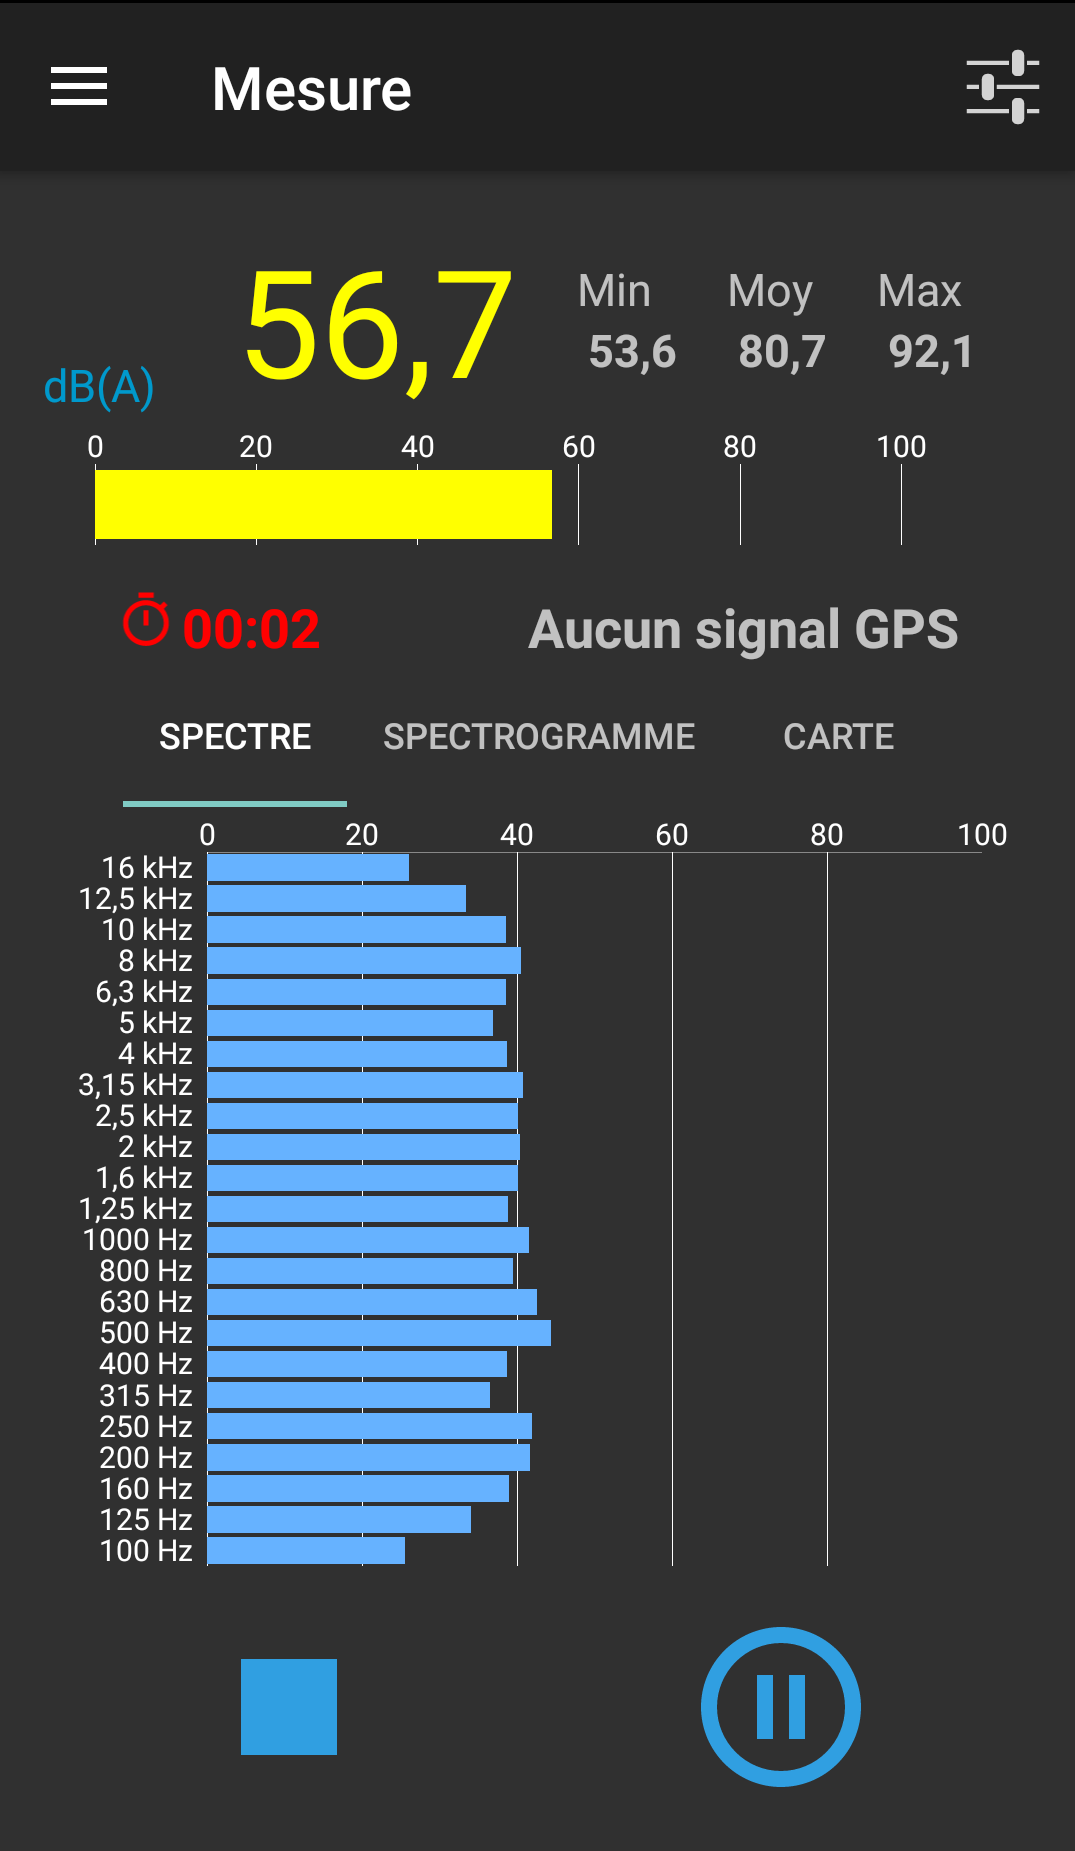
\includegraphics[width=0.9\textwidth]{./figures/autres/noiseCapture1.png}
    \end{minipage}
    \begin{minipage}[t]{0.3\textwidth}
        \centering
        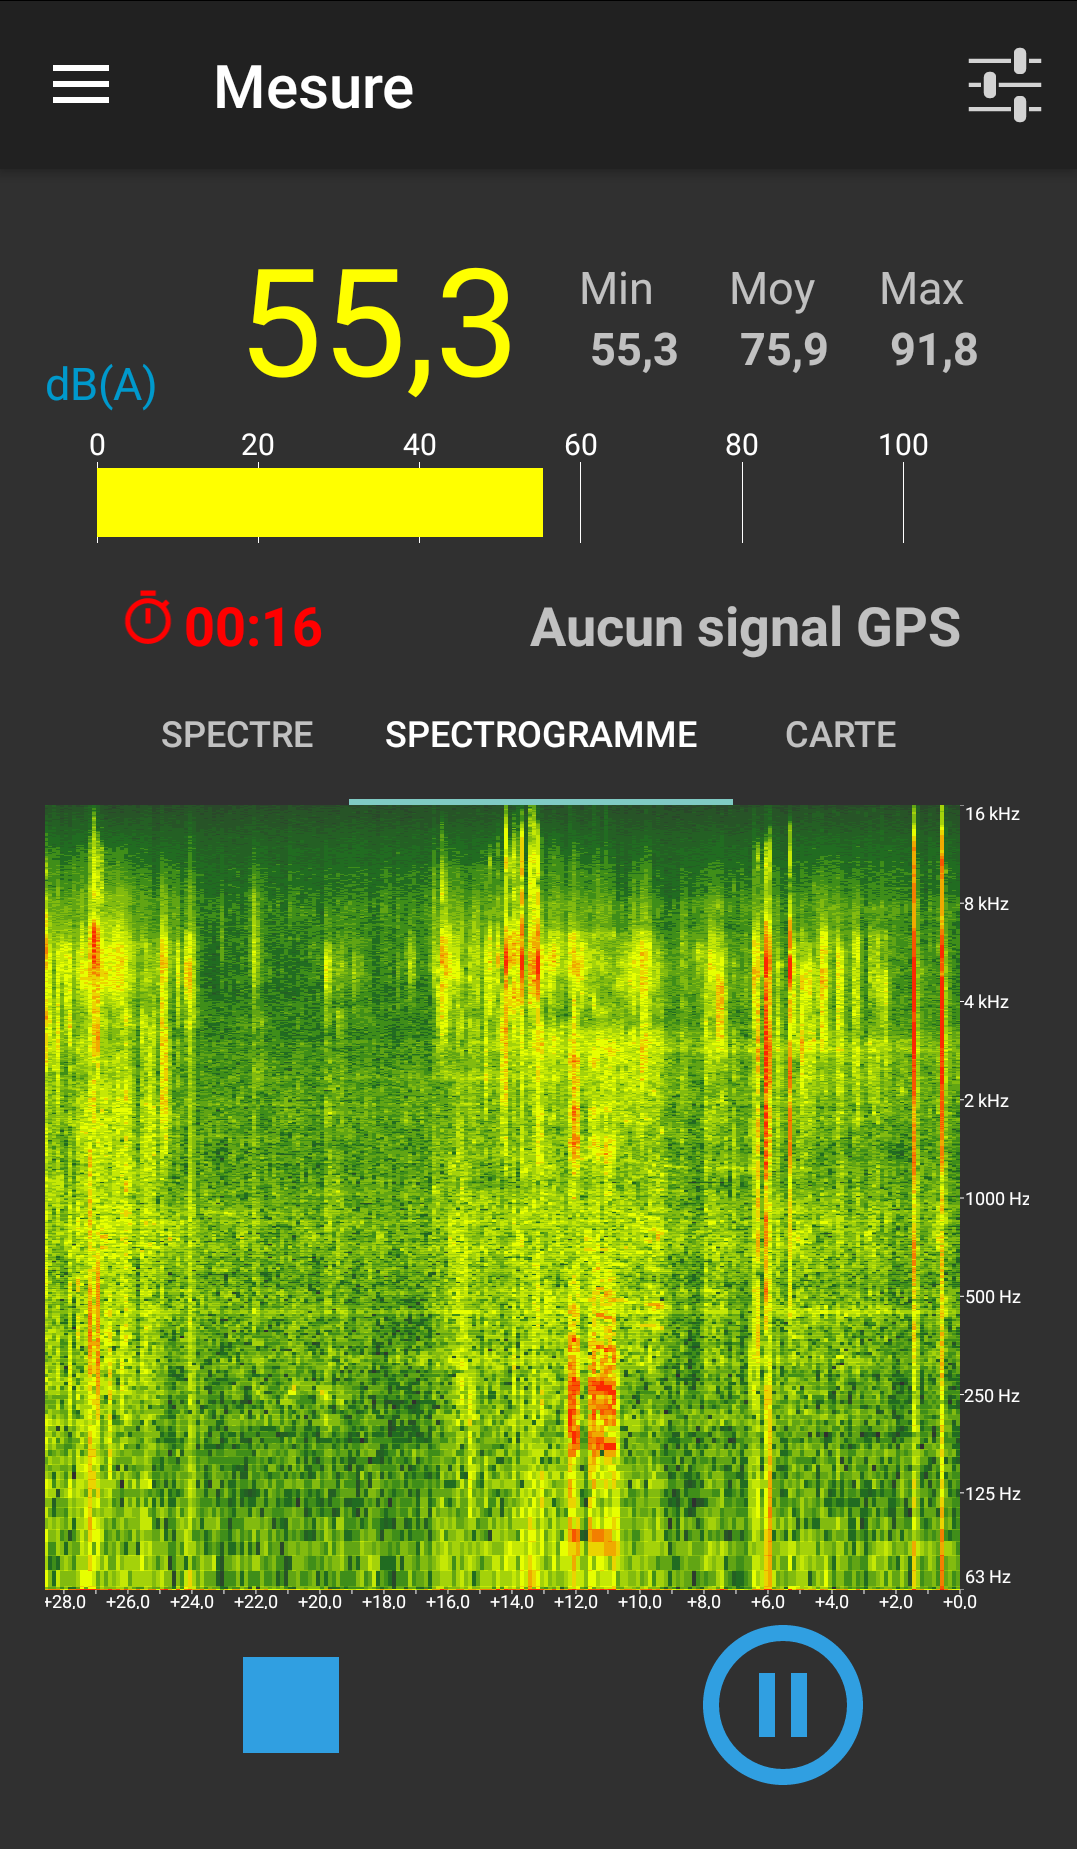
\includegraphics[width=0.9\textwidth]{./figures/autres/noiseCapture3.png}
    \end{minipage}
    \begin{minipage}[t]{0.3\textwidth}
        \centering
        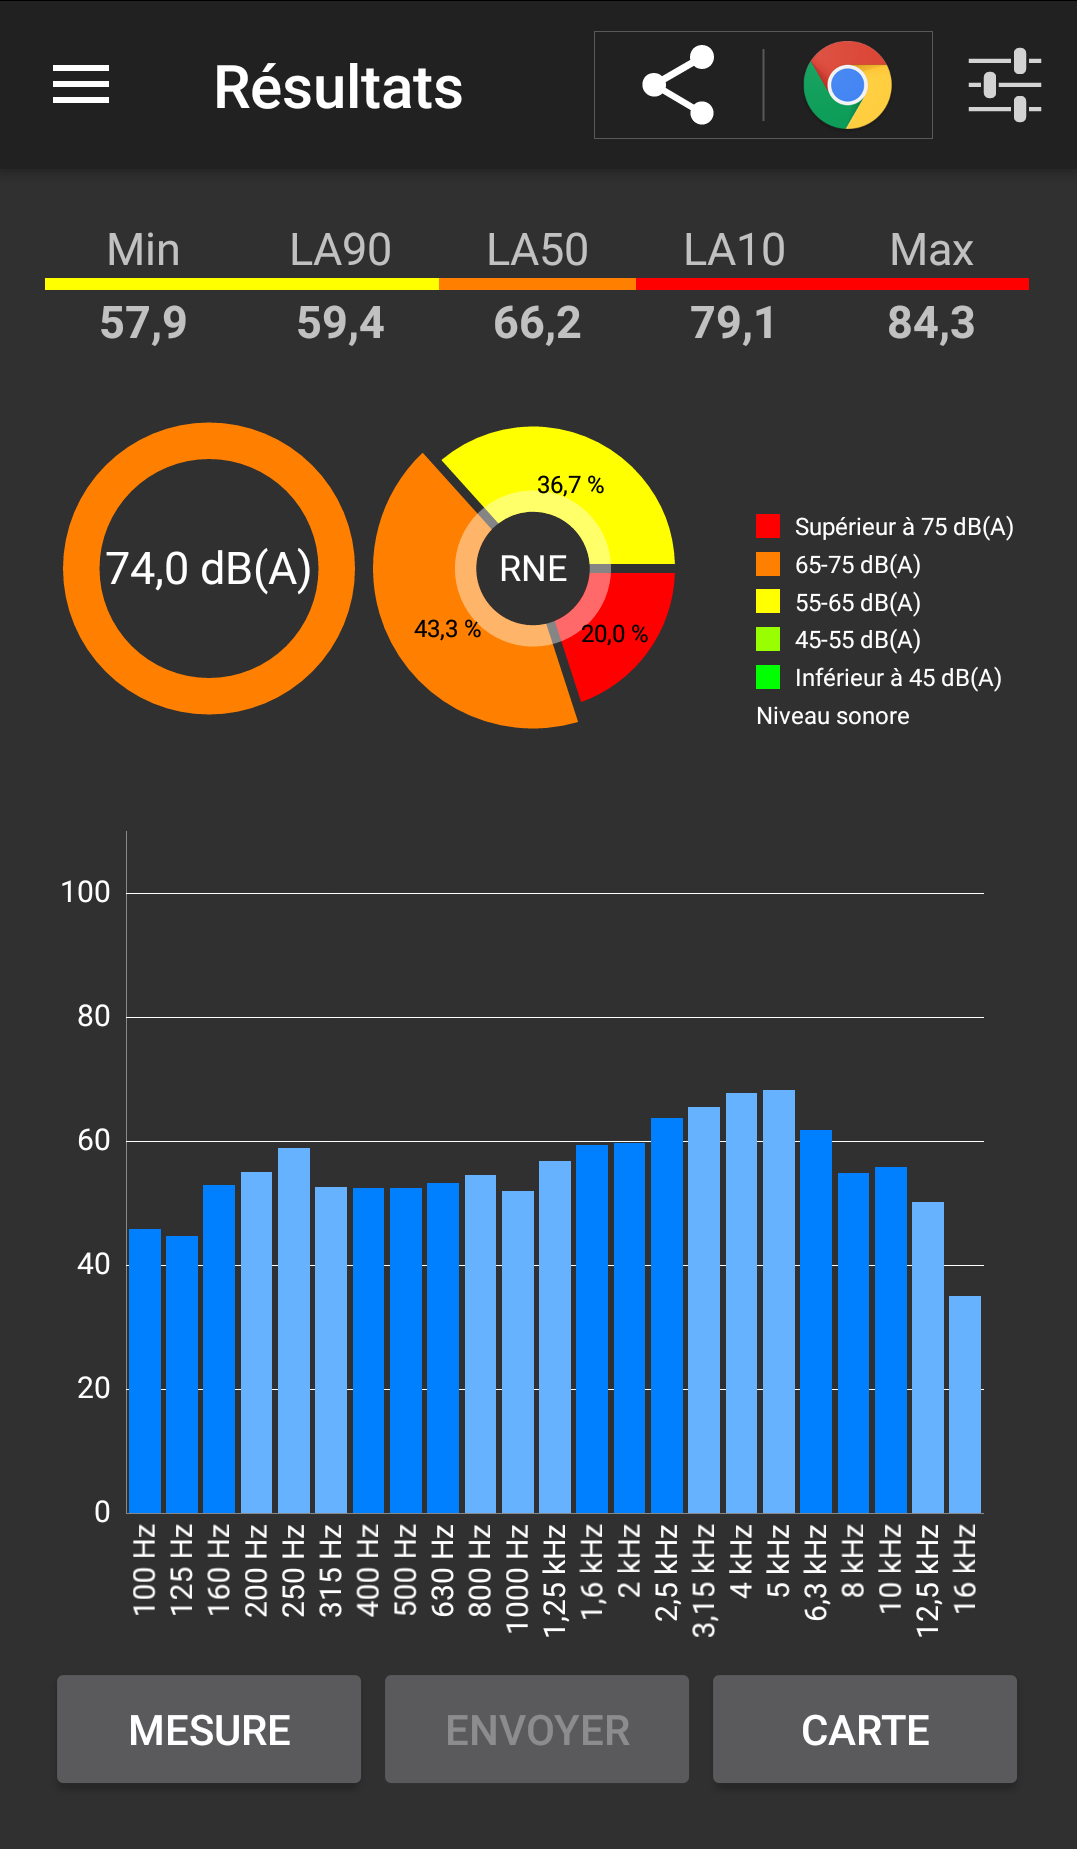
\includegraphics[width=0.9\textwidth]{./figures/autres/noiseCapture2.png}
    \end{minipage}
    \caption{Captures d'écran de l'application \textit{NoiseCapture}}
\end{center}
\end{figure}


\begin{figure}[t]
\centering
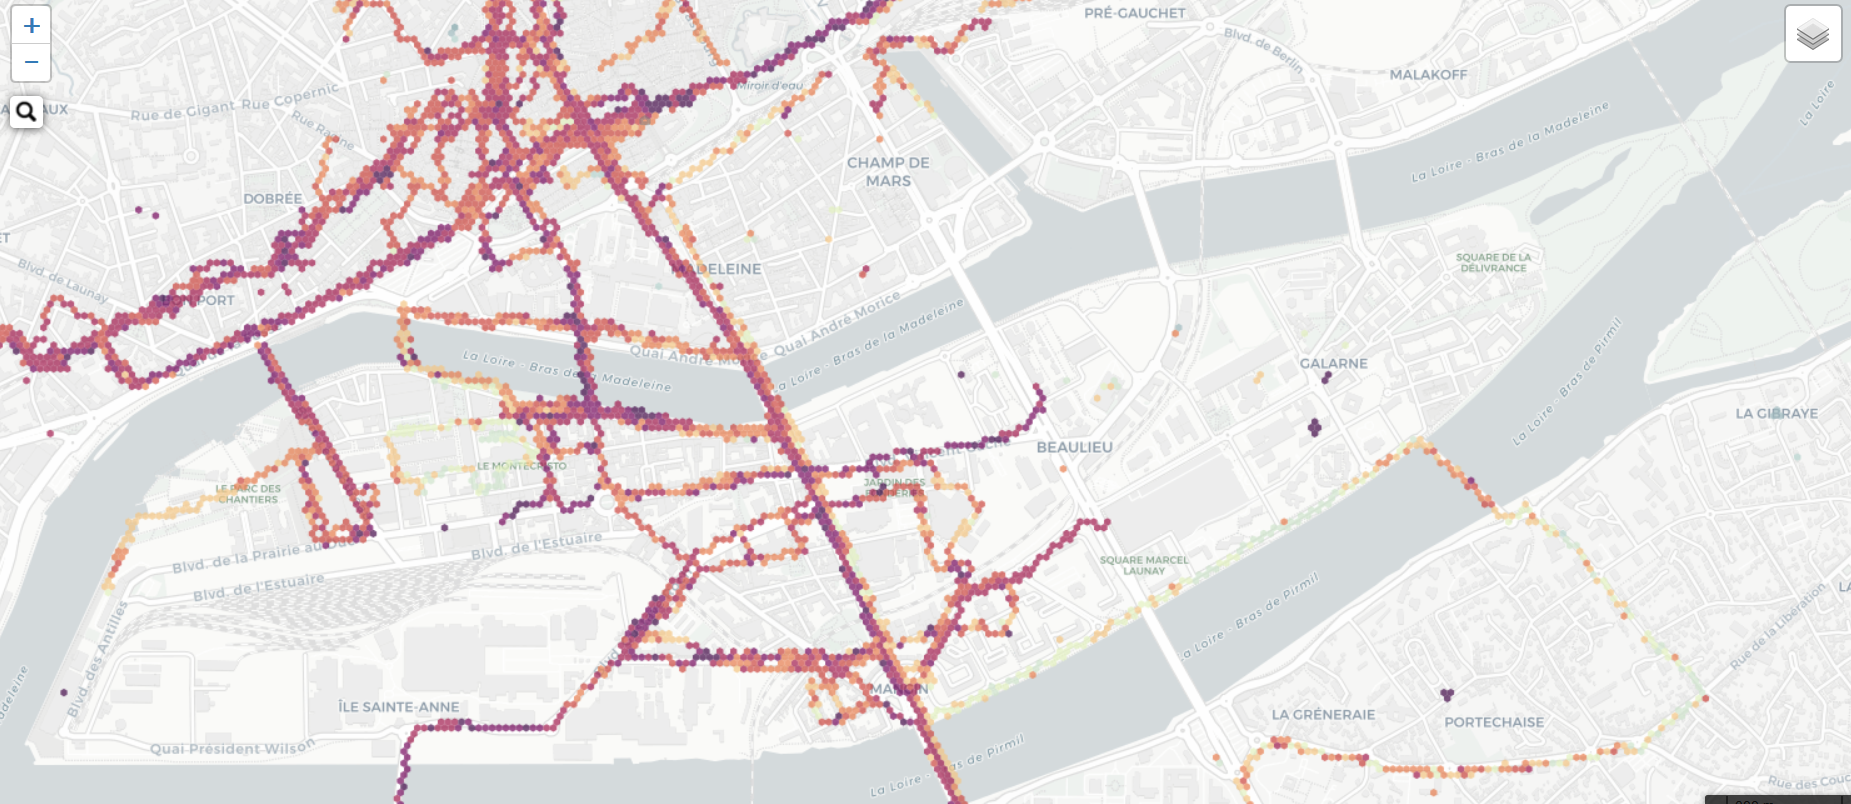
\includegraphics[width=0.7\linewidth]{./figures/cartographie/noise_modelling.PNG}
\caption{Carte de l'ESU de l'île de Nantes mesurée par l'application \textit{NoiseCapture}  (relevée le 22/03/2018)}
\label{fig:carte_noiseModelling}
\end{figure}


\section{De l'extraction d'informations des mesures}

Là où l'approche par modèles prédictifs suppose l'utilisation de modèles d'émissions sonores pour chaque source, l'utilisation de mesures acoustiques, dans le cadre de l'étude des ESU, permet : 
\begin{itemize}
\item d'estimer la contribution \textit{in situ} du trafic routier pour, au minimum, valider les modèles des prédiction de bruit de trafic ou, au mieux, pouvoir estimer le niveau sonore du trafic plus précisément et finement,
\item de considérer l'ensemble des sources sonores présentes afin de caractériser les ESU dans leur globalité,
\item et de s'orienter vers la cartographie multi-sources par l'estimation des contributions de sources sonores spécifiques pour ainsi mieux considérer la perception du citadin.\\
\end{itemize}

Toutefois, comme tout signal mesuré, il est nécessaire de disposer d'outils adaptés afin d'y déterminer les informations utiles.

En effet, l'ESU est un milieu complexe composé d'une multitude de sources variées (trafic routier, voix, oiseaux, klaxon, bruit de pas\dots). Ces sources ont des allures temporelles différentes parfois brèves (le retentissement d'un klaxon) ou longues (le passage d'une voiture) ainsi que des allures spectrales variées (dans les basses fréquences pour le trafic, dans les hautes fréquences pour le sifflement des oiseaux), voir Figure \ref{fig:sourceUrbain}. L'ensemble de ces sources est aussi susceptible d'être généré simultanément. La création d'outils adaptés à cet environnement pour reconnaitre ou détecter des sources spécifiques n'est donc pas triviale. Par exemple, dans le cas du trafic routier, s'il existe des endroits où celui-ci est prépondérant sur les autres sources sonores (périphérique, grand boulevard), il peut l'être moins dans d'autres lieux (dans des rues calmes, au niveau de parc) où ce sont d'autres sources sonores qui sont majoritairement présentes (voix, oiseaux \dots). Considérer l'ensemble des mesures et des enregistrements réalisés en ville sans distinction particulière entre les sources peut donc mener à de mauvaises estimations du temps de présence ou de son niveau sonore et donc à de mauvaises interprétations. 

\begin{figure}[t]
\centering
\subfigure[\label{fig:sourceUrb1}]{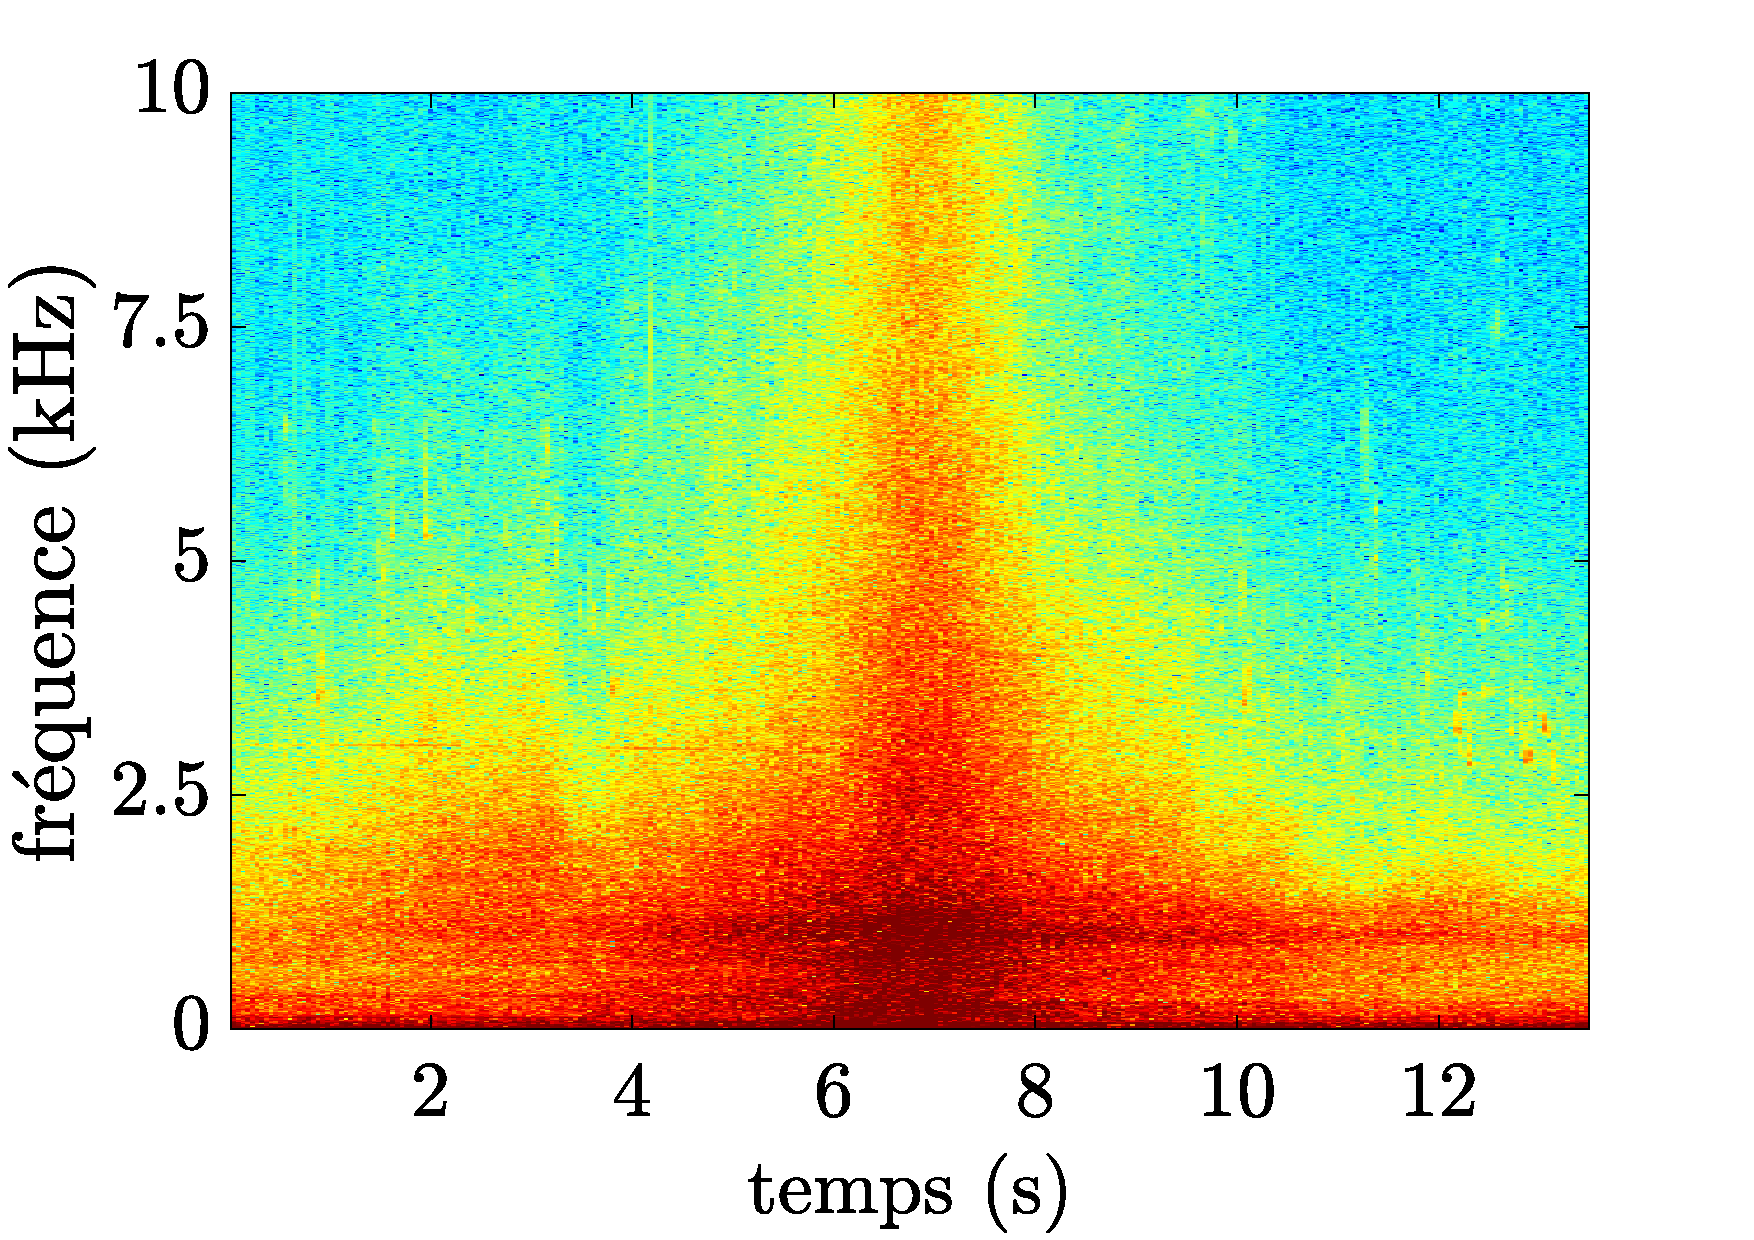
\includegraphics[width=0.4\linewidth]{./figures/autres/sourcesUrbainesCar.pdf}}
\subfigure[\label{fig:sourceUrb2}]{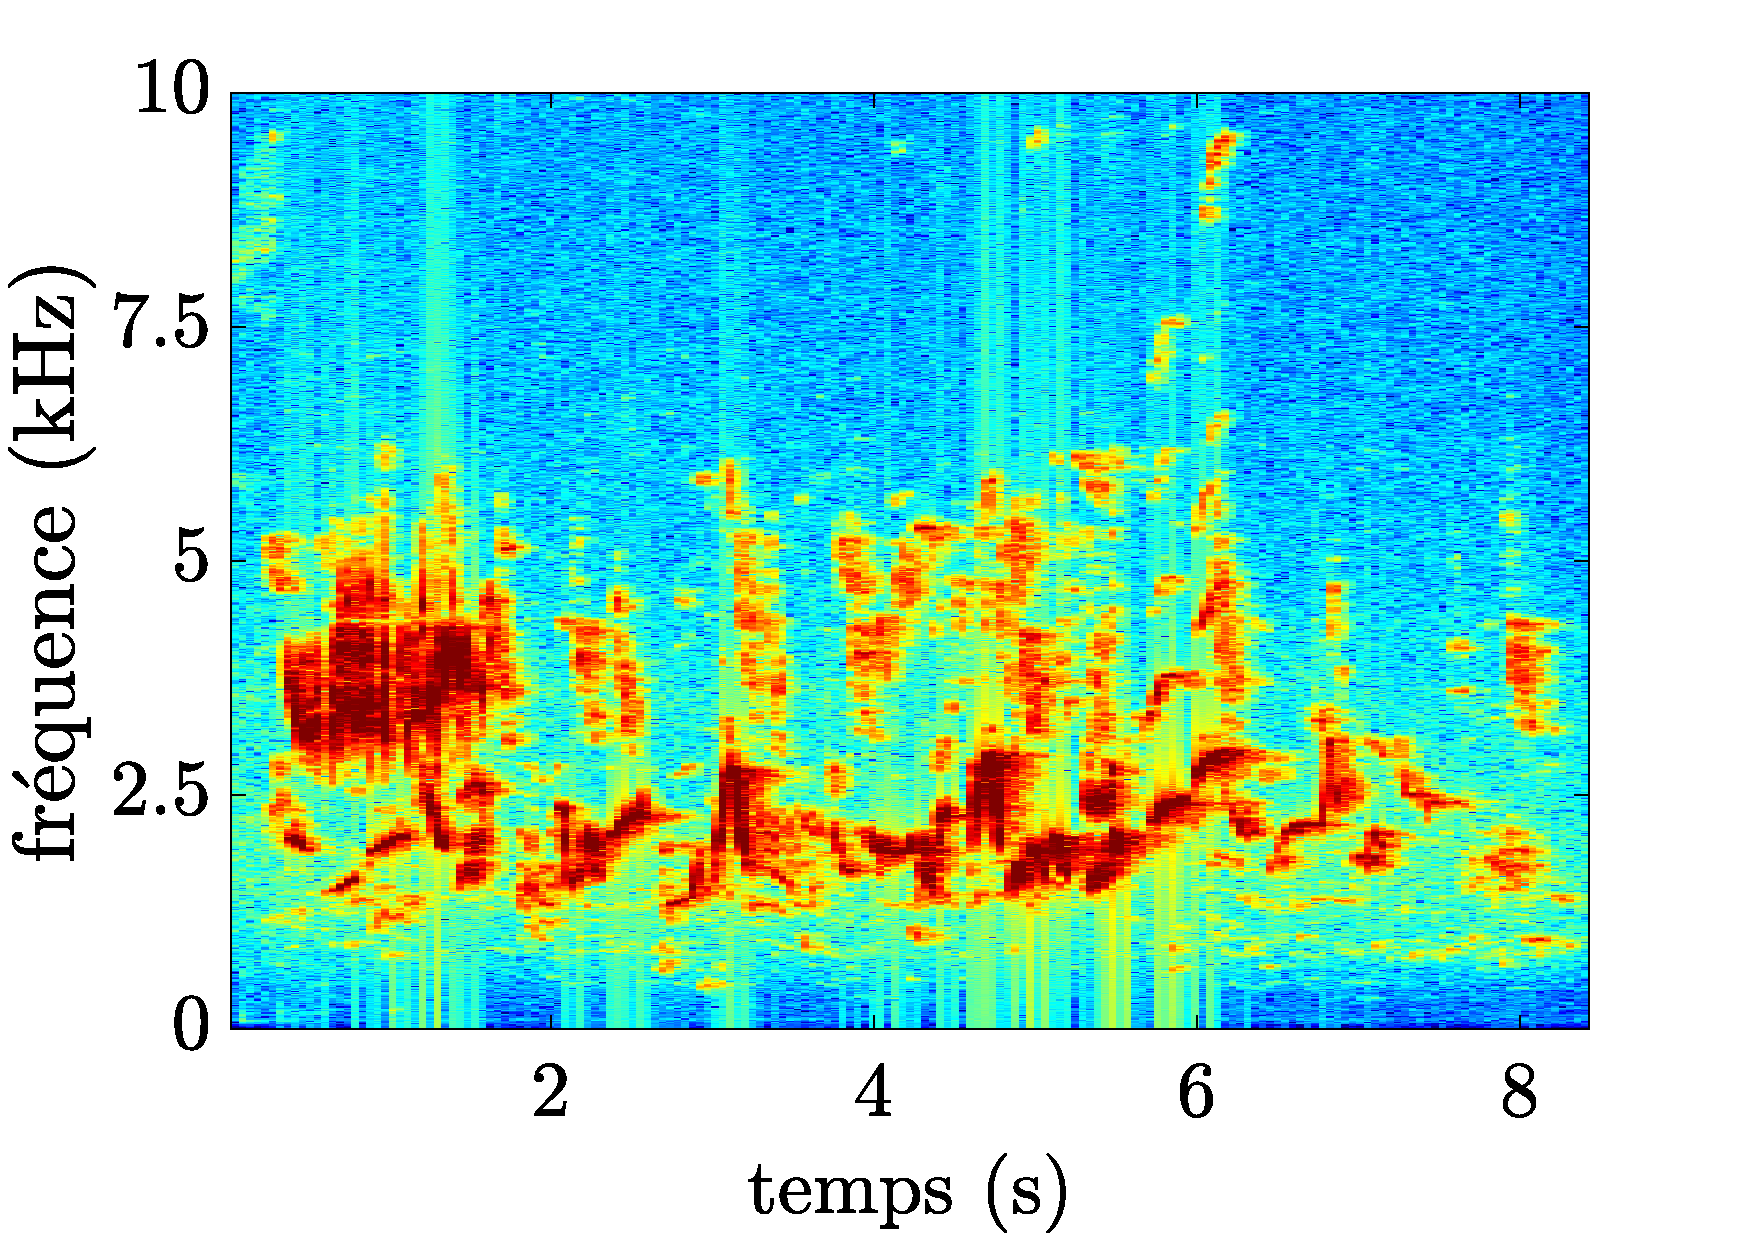
\includegraphics [width=0.4\linewidth]{./figures/autres/sourcesUrbainesBird.pdf}}
\subfigure[\label{fig:sourceUrb3}]{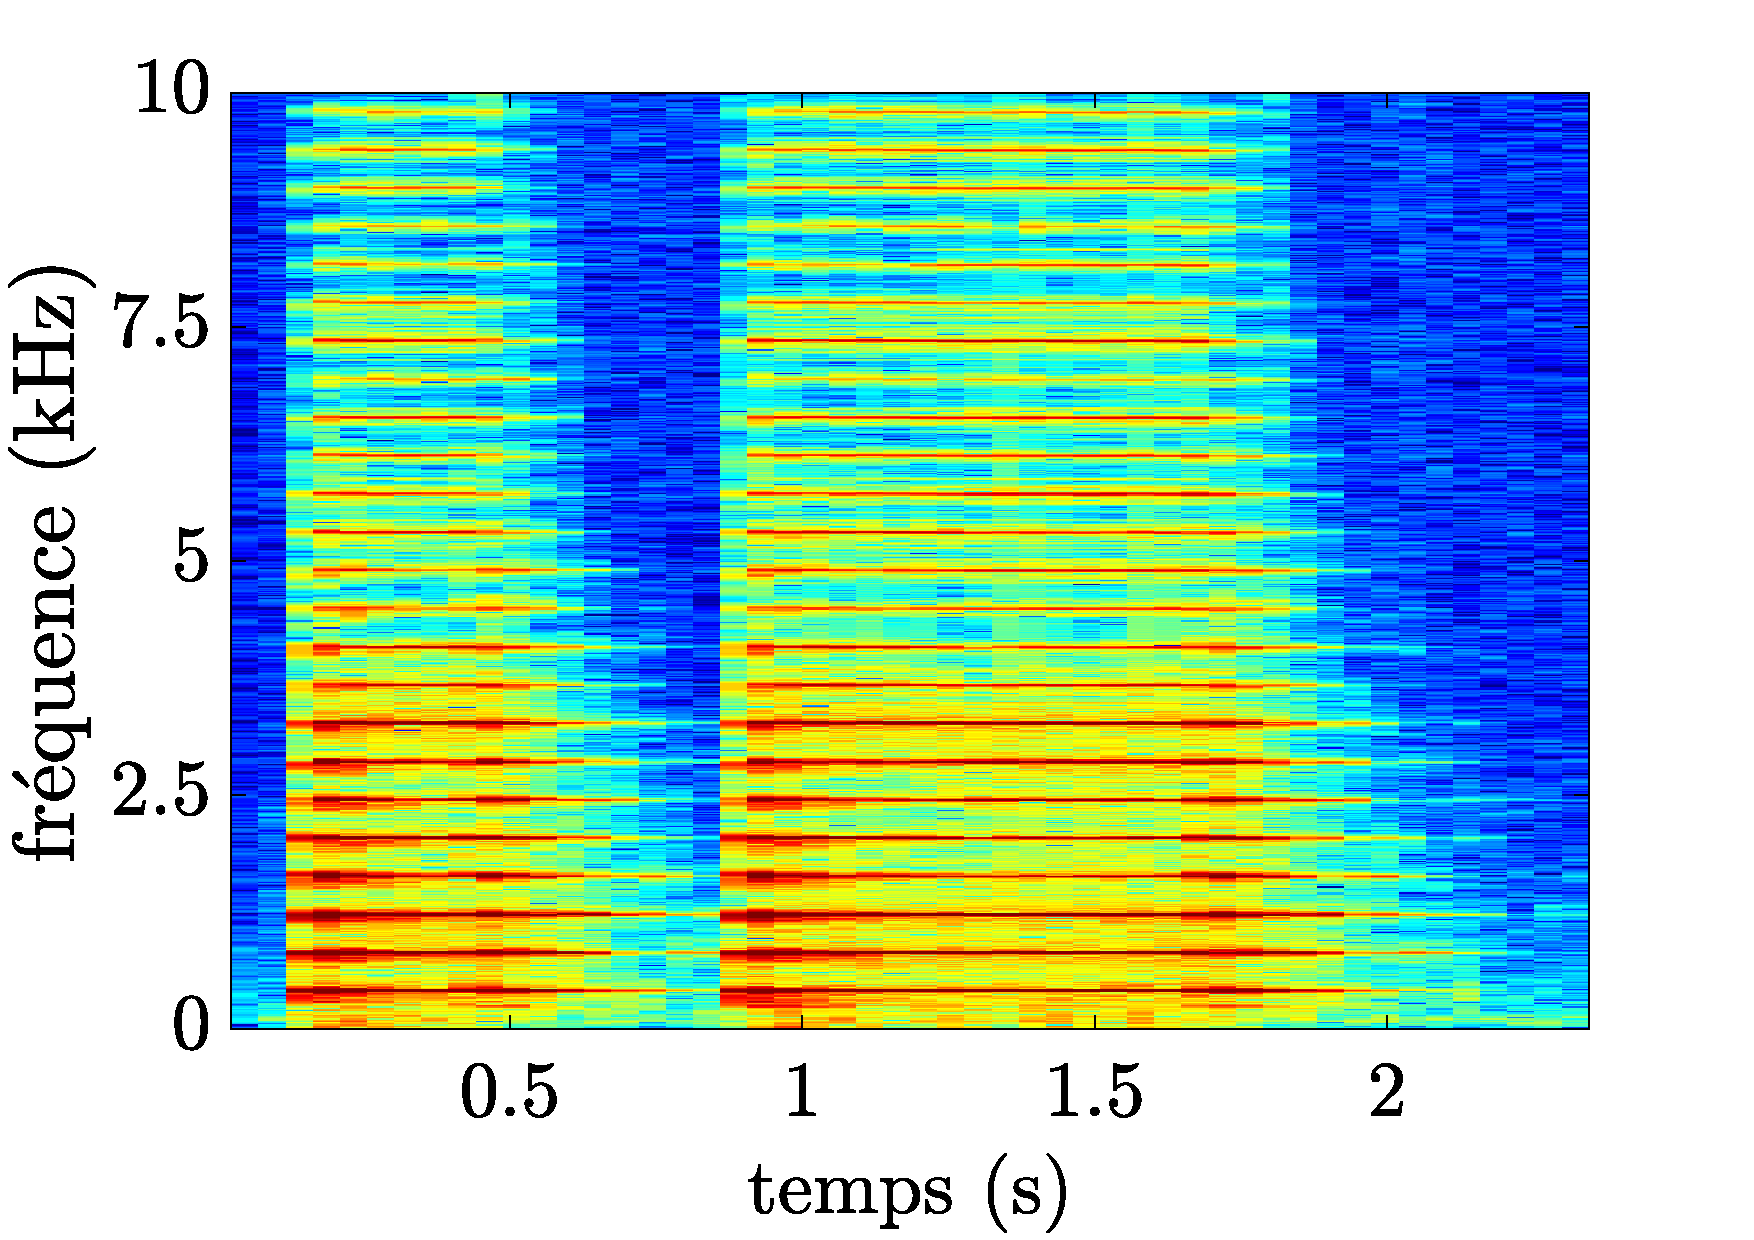
\includegraphics [width=0.4\linewidth]{./figures/autres/sourcesUrbainesCarHorn.pdf}}
\subfigure[\label{fig:sourceUrb4}]{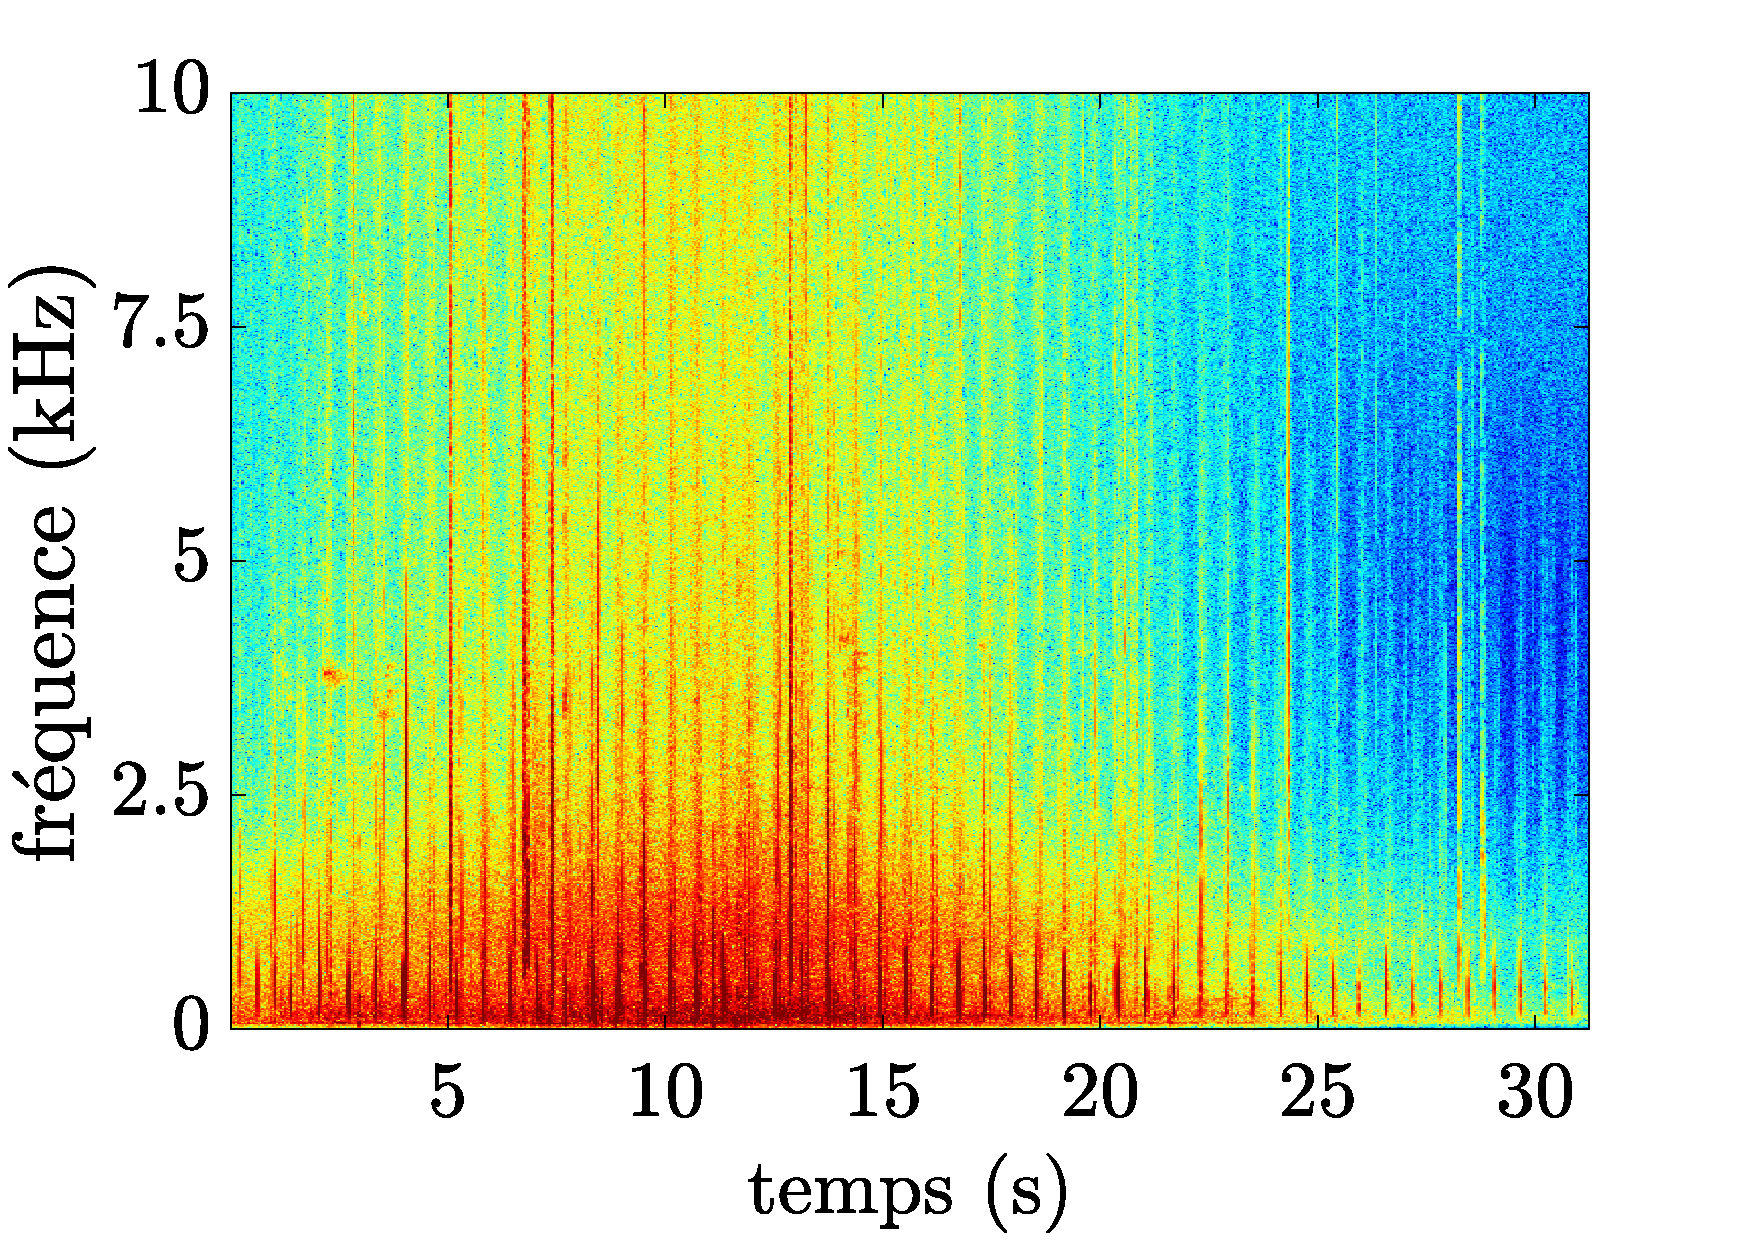
\includegraphics [width=0.4\linewidth]{./figures/autres/sourcesUrbainesFootStep.pdf}}
\caption{Spectrogrammes d'un passage d'une voiture \subref{fig:sourceUrb1}, d'un sifflement d'oiseaux \subref{fig:sourceUrb2}, d'un klaxon \subref{fig:sourceUrb3} et d'un bruit de pas \subref{fig:sourceUrb4}.}
\label{fig:sourceUrbain}
\end{figure}


Dans \cite{Mioduszewski}, la réalisation de mesures par 40 stations fixes durant 1 an révèle que les niveaux sonores mesurés sont supérieurs à ceux estimés par les modèles prédictifs. Une part de cette surestimation provient de la prise en compte des bruits qui ne sont pas relatifs au trafic  mais aussi des modèles prédictifs qui ne permettent pas d'inclure les bruits provoqués par des véhicules pouvant se garer à proximité des capteurs. Ses travaux révèlent donc la nécessité de générer un outil adapté à l'étude des mesures et enregistrements faits en villes pour y extraire les contributions et les niveaux sonores des sources présentes en villes.\\

En conséquence, les travaux de cette thèse cherchent à répondre à ces questions : 
\begin{itemize}
\item \textbf{Comment déterminer le niveau sonore des sources en villes ?}
\item \textbf{Quelles sont les méthodes disponibles pour réaliser cette tâches ?}
\item \textbf{Quel protocole expérimental mettre en oeuvre pour tester et valider les performances de ces outils ?}
\end{itemize}


\section{Estimation du niveau sonore du trafic routier à partir de mesures}

\subsection{Objectifs}
Étant la source principale de bruit en ville ainsi que la plus gênante, le trafic routier sera la source d'intérêt qui sera principalement étudié. 

nous nous intéressons à l'estimation du niveau sonore du trafic routier à partir d'enregistrements sonores.
Cette problématique non traitée va consister à appliquer une méthode de 
Appliquer un traitement sur le signal d'enregistrement (44,1 kHz en format wav).

\subsection{Protocole expérimental}

Extraire le trafic routier par des méthodes de séparation de sources, d'autre méthodes existent mais on retient celle là pour des raisons explicité plus tard

\begin{figure}[t]
\centering
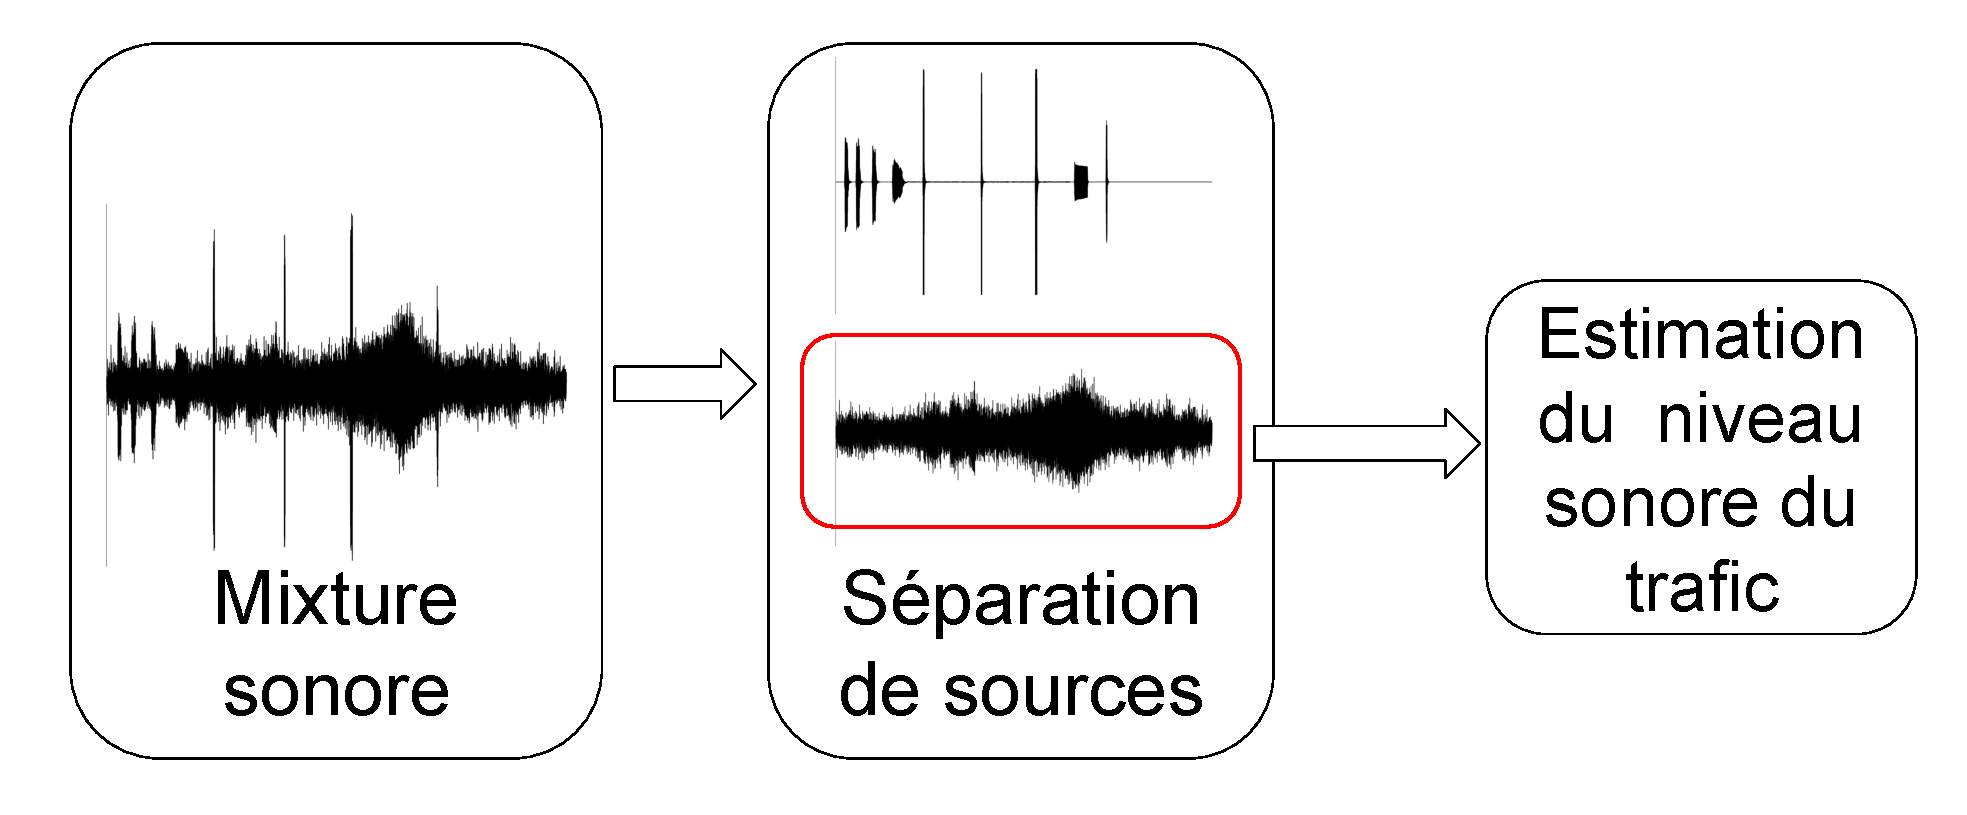
\includegraphics[width=0.7\linewidth]{./figures/NMF/bloc_diagram_source_separation.pdf}
\caption{Diagramme bloc de l'approche par séparation de sources.}
\end{figure}


Pour cela, l'utilisation d'enregistrement n'est pas possible puisque le niveau sonore du trafic réel est l'inconnu qu'on cherche. Dans le cas où il n'y a que du trafic, l'estimation fournie par la méthode peut être comparé mais quid des scènes sonores où le trafic n'est pas prépondérant et que d'autres sources sonores recouvrent cette composante ?
Le choix est donc fait d'appliquer la méthode de séparation de sources sur des scènes sonores simulées le plus réaliste possible. Cet aspect réaliste est primordiale afin de donner un sens et une validité aux résultats émis par la méthode.\\


Les scènes sonores étant simulée, un contrôle total des classes sonores présentes et de leur niveau sonore est alors possible. Les niveaux sonores exacte en dB sur la globalité de la scène pour chaque classe de son est ensuite disponible, dont le trafic, $L_{eq,trafic}$. En appliquant la méthode de séparation, la composante trafic est extraite du signal et son niveau sonore, $\tilde{L}_{eq,trafic}$, est estimé. La figure \ref{fig:diagramBlocProtocol}.

\begin{figure}[t]
\centering
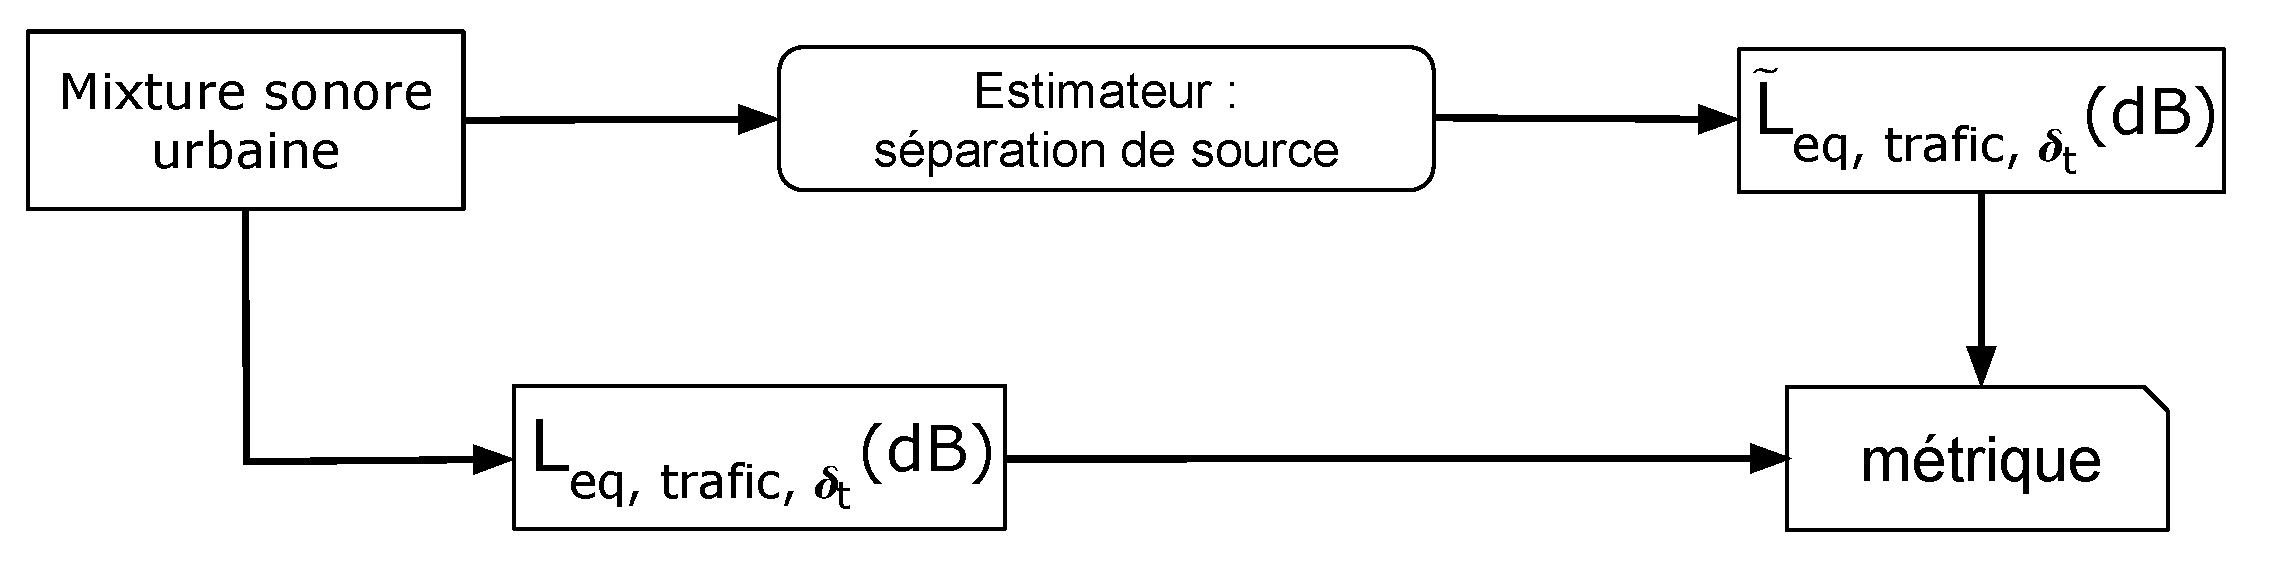
\includegraphics[width=0.7\linewidth]{./figures/NMF/Bloc_diagram_estimateur_FR.pdf}
\caption{Diagramme bloc du protocol expérimental.}
\label{fig:diagramBlocProtocol}
\end{figure}


Une métrique est alors choisie pour déterminer l'erreur moyenne produite sur un ensemble de $M$ scènes testés. Parmi les différentes métrique possible (somme des carrés des résidus $SCR$, racine de l'erreur quadratique moyenne $RMSE$), l'erreur absolue moyenne, $MAE$ (pour \textit{Mean Absolute Error}) est retenue,  

\begin{equation}
MAE = \frac{\sum_{i = 1}^{M} \vert L_{eq, trafic}^i - \tilde{L}_{eq, trafic}^i \vert}{M}.
\end{equation}

Contrairement à l'erreur RMSE, qui revient à la racine carré de la moyenne du carré des différences entre les données observées et réelles, qui pénalise plus les valeurs qui défie fortement, l'erreur $MAE$ présente l'intérêt de considérer un poids identique entre chaque différence et ainsi de gagner en interprétabilité.\\

Ces travaux se concentre sur l'estimation du signal du trafic routier tant elle est la source de bruit principale et la plus gênante. Toutefois, l'estimation d'autre signaux acoustique en ville est naturellement possible à partir de mesures acoustiques ou d'enregistrements en vue de détecter d'autres classes de sons spécifiques ou à l'étude plus générale de l'ESU.




%
%%\bibliographystyle{unsrt}
%%\bibliography{../bibliographie}
%%
%%\end{document} 
%
%%\subsection{Incertitudes liées à la modélisation numérique}
%%
%%Les cartes de bruits étant simulées, des problèmes apparaissent également lié à la modélisation et à la discrétisation du milieu urbain. Afin de limité la durée des calculs de techniques d'optimisation sont utilisées comme la discrétisation du milieu mais aussi des sources de bruits. Par exemple, pour une route décrite comme une source linéique de bruit, celle est discrétisé en un ensemble de source ponctuel alignées. Le choix de la distance entre ces points est alors un compromis à faire entre temps de calcul et précision souhaitée. Toutefois la position de ces sources influe ensuite sur les phénomènes de réflexion et de diffraction. De plus, afin de réduire les temps de calculs, les niveaux sonores entre les points calculés sont déterminés au moyen d'un calcul d'interpolation (méthode de Krigeage) qui viennent donc rajouter en plus des incertitudes \cite{van_leeuwen_noise_2015}. 
%%
%%IMAGE d'INTERPOLATION ?
%%
%%Enfin toujours en raison de la limitation des moyens numériques, l'effet de l'architecture urbaine (balcon, fenêtre) ou du mobilier urbain n'est pas pris en compte dans la modélisation des villes car trop complexe à réaliser alors que ces éléments ont un impact qui n'est pas pris en compte. 
%%
%%\subsection{Représentation des données et estimation du nombre de citadins touché}
%%
%%Une fois les cartes produites, indépendamment des remarques faites précédemment, une des critiques quant aux cartes de bruits est la limitation d'informations qu'elle produisent : un niveau sonore $L_{DEN}$ et $L_N$ pour décrire le niveau sonore du trafic. Ces deux seules indicateurs permettent certes d'avoir un aperçu global d'une grandeur qui, pourtant, évolue constamment. En effet, aussi bien à l'échelle de l'année ou d'une journée, le trafic routier évolue sans cesse. Cette évolution peut se diviser en 4 parties : un pic de trafic situé entre 7h et 9h et entre 16h et 18h correspondant au moment où les citadins emprunte leur voiture pour se déplacer entre leur domicile et leur travail. Entre ces 2 périodes, la quantité de voiture est plus faible \cite{}. La prise en compte ces évolutions de débit de trafic dans les modèles afin de simuler des cartes heures par heures est toutefois compliqué à mettre en œuvre car elle nécessiterait de grande quantité de ressources informatiques et cette approche ne permettrait pas d'obtenir l'évolution annuelle.
%%Coupler les modèles de sources et de propagation à des modèles dynamiques de trafic est une voie pour créer des cartes de bruit de trafic dynamiques prédictives. 
%%
%% Dans \cite{modiuszeski}, Modiuszeski compare le niveau sonore simulée prédit par la carte de bruit avec les résultats de mesures réalisée toute l'année. Il constate alors aisément que l'évolution des niveaux sonores évolue autant à l'échelle de la journée que de l'année rendant les valeurs $L_{DEN}$ et $L_N$ extrêmement restrictives. Enfin, au fur et à mesure que la perception du citadin de l'environnement sonore est mieux connu, il a été montré que les indicateurs de niveaux sonores du trafic pondéré A n'est pas suffisant pour rendre compte de sa perception de l'environnement sonore. Selon, le cadre architecturale de la ville, le statu social du citadin et les sources sonores présentes, pour un niveau sonore trafic similaire, l'agrément de l'ambiance sonore par le citatdin eut ne pas être la même. En conséquence, à partir des études sur le \textit{soundscape} \cite{schafer_soundscape_1993}, il peut être envisagé de réaliser des cartes de bruits, non plus liées à une seule source de bruit, mais à la perception du citadin de l'environnement sonore (\og agréable \fg{}, \og très désagréable \fg{}, \dots). Ces cartes ne se feraient plus alors à partir d'une source de bruit mais sur l'ensemble des sources sonores présentes dans les zones et permettraient, au citadin, de savoir si tel quartier a un environnement sonore agréable ou non.\\
%%
%%Des indicateurs de niveaux sonore, le nombre de citadins exposés au bruit peut être déterminé. Là encore, la méthode pour estimer ce chiffre est discutable. King et Murphy résument cela dans un paragraphe dans \cite{king_implementation_2011}. L'hypothèse faite est que les individus vivent et dorment toute l'année au niveau de la façade la plus exposée, ce qui n'est pas forcément représentatif de la réalité. Cette hypothèse conduit notamment à une surestimation du nombre de personnes touché par des niveaux sonores. \\
%%
%%La réalisation de ces cartes visant à diminuer l'exposition des citadins au forts niveaux sonores, les incertitudes provoquées par les différents étapes peuvent entrainer la mise en chantier d'un plan d'action mal adapté à la situation réelle. Mais l'amélioration des cartes, telles qu'elles sont faites actuellement, semble toutefois limité : l'augmentation de la résolution des permettrait bien de corriger certaines erreurs dû aux interpolations mais viendrait à augmenter considérablement les cout de calculs. De plus, ce choix rendrait impossible de mettre à jours les cartes régulièrement pour prendre en compte les fluctuations du trafic à l'échelle de l'année ou même encore durant la journée. En conséquence, à l'heure où les villes s'équipent en réseaux de capteurs (météorologique, qualité de l'air) en vue de devenir des \og villes intelligentes \fg{} (\textit{smart cities} en anglais), il devient possible d'ajouter des capteurs acoustiques afin de s'en servir pour décrire l'environnement sonore urbain. \\
%


%\subsection{Détection d'évènements sonore spécifiques}
%
%Plusieurs études se sont intéressées à la détection d'évènements particuliers en lien avec la sécurité. Par exemple, la détection acoustique de la sirène d'une ambulance est envisageable à partir d'un réseaux de capteurs \cite{schroder2013automatic,karpis2012system} ou bien de coups de feu ou d'explosifs \cite{showen1999automatic,simon_sensor_2004}.  
%Pour aller plus loin, \cite{foggia_audio_2016} propose de coupler des capteurs acoustiques à des caméra vidéo afin de faciliter la détection d'accident de la route. 



%\subsection{Cartographie des ESU}
%
%D'autres études se sont intéressées aux ESU de manière plus générale afin de classifier les environnements sonores par ambiance à partir de différents indicateurs physiques comme dans \cite{can_describing_2015} où le niveau sonore équivalent pondéré $A$, son écart type et le centre de gravité spectrale entre les bandes de 50 Hz et 10 kHz sont considérés pour discriminer les ambiances sonores. Dans \cite{salamon2015unsupervised}, Salamon et Bello utilisent un algorithme de k-moyenne sphérique en tant que classifieur. 
%La cartographie de l'ESU selon des ambiances sonores défini (\textit{parc}, \textit{rue piétonne}, \textit{boulevard} \dots) est alors possible pour offrir une autre représentation de la ville lié non pas à une source sonore spécifique mais à la somme des différentes sources présentes sans distinction entre elles.  

%Une autre piste à l'étude est la description des ESU à travers la perception du citadin \cite{brocolini_measurements_2013}.
%Cette approche est résumée sous la notion de paysage sonore (ou \textit{soundscape} en anglais). Proposée par R. Murray Schafer \cite{schafer1977tuning}, cette notion considère que la perception de l'ESU par le citadin est liée à sa construction sociale (âge, expérience, milieu social\dots), là où l'ESU est le résultat de phénomènes physiques (source sonores, diffusion du son, réverbération\dots). 

%En conséquence, plusieurs études se sont intéressées à l'évaluation de l'ESU aux travers de descripteurs acoustique sémantiques (Evaluation de la scène, clarté, occupation spatiale, évolution temporelle)  \cite{raimbault2003ambient,hall2013exploratory}, afin de définir les éléments (sources sonores, environnements) qui sont les plus gênants ou bien les plus appréciés. 
%D'autre études, en vue de prédire le paysage sonore, lient la perception de l'ESU à des indicateurs physiques (niveau sonore pondéré, niveau sonore fractile $L_x$\dots). Ces modèles prédictifs peuvent être établi à partir d'écoutes réalisées en laboratoire comme dans \cite{torija2013application} où le paysage sonore est décrit à partir de 14 indicateurs dont le facteur crête (rapport du niveau sonore maximum sur le niveau sonore équivalent à 15 minutes), le niveau sonore pondéré $A$ des signaux contenant une réponse impulsionnelle ou les niveaux sonores des bandes de tiers d'octave de 125 Hz et 16 kHz.
%Il est également possible de réaliser des marches sonores en ville (ou \textit{soundwalk} en anglais). Cette approche consiste à faire évaluer l'ESU à des auditeurs le long d'un parcours effectué en ville. Intiallement proposée par \cite{southworth1967sonic}, la réalisation de \textit{soundwalk} a ensuite été popularisée par R. M. Schafer dans le concept du \textit{soundscape} où sa pratique est centrale dans l'étude de l'ESU \cite{schafer1969new, schafer1977tuning}. Ces marches présentent l'avantage de permettre une représentation du monde plus réaliste que des écoutes en laboratoire et ainsi une meilleure validité écologique. Mais, les \textit{soundwalks} restent tributaires des sources sonores présentes dont le niveau sonore et la présence ne sont pas controlables. Ces études sont donc plus difficilement généralisables que celles réalisées en laboratoire. 

%Dans \cite{hong2014soundscape}, des cartes du paysage sonore urbain sont réalisées, à l'aide d'un logiciel SIG, à partir de l'évaluation perceptive de la présence du trafic, des sons technologiques, des sons humains et des sons naturels ainsi que de l'évaluation du paysage sonore et de l'environnement urbain. Ces évaluations sont complétées par un seul indicateur physique, le niveau sonore équivalent pondéré $A$, $L_{A,eq}$. Cette étude révèle que le bruit de trafic perçu est corrélé au $L_{A,eq}$ alors que les sons naturels (sifflement d'oiseaux, bruit de fontaine) ne le sont pas (corrélation négative). Dans \cite{aumond2017modeling}, c'est la notion d'agrément sonore qui est défini (ESU plaisant ou déplaisant) à partir de deux modèles : l'un perceptif et l'autre physique. Le modèle perceptif est établit à partir du niveau sonores globale et du temps de présence de plusieurs source sonore spécifiques : trafic, voix, et oiseaux. Le modèle physique est basé sur des indicateurs physiques tels que le niveau sonore fractile $L_{50}$ dans la bande de tiers d'octave de 1 kHz ainsi que la variation normalisée en temps et en fréquence des bandes de 500 Hz et de 4 kHz. Ces indicateurs permettent de traduire la présence des sources sonores du modèle perceptif. 

%De ces différents modèles, réaliser des cartes de l'ESU perçu à partir des mesures issus des réseaux de capteurs serait alors envisageable et permettraient d'apporter une autre représentation de l'environnement sonore de la ville basée sur la perception du citadin et non sur les niveaux sonores physiques prédits des sources sonores les plus gênantes.
